\documentclass[british,titlepage,oneside]{project_setup}

\addbibresource{bibliography.bib}

\input{glossary.tex} % add glossary and acronym lists before document

\begin{document}
\setstretch{1.2}

\chapter*{Abstract}
\begin{comment}
A condensation of the essential information of the article.
\end{comment}

Autonomous navigation in increasingly complex domains presents new challenges that question the efficiency and capability of traditional model-based methods. Though traditional approaches have been successful for unstructured environments in the past, uncertain, sensor-degraded, or dynamic environments cannot be modelled and thus be solved by these approaches. Instead, learning-based methods have become increasingly popular due to their ability to learn complex behaviour without explicit programming, where multiple components can be combined into a single model to tackle the perception, prediction and motion task of autonomous navigation.

In this theme, this thesis explores the use of reinforcement learning for autonomous navigation of a quadrotor through cluttered environments, with only a depth camera. We propose a two-part deep neural network model comprised of an encoder-CNN and MLP, where the CNN serves as the perception module while the MLP is the optimal controller. With this framework, our model receives a quadrotor state and depth image as input and maps this to a velocity and yaw rate reference to reach a specified goal in three dimensions.

To solve the task, we present the problem as an unsupervised representation learning and reinforcement learning task. The CNN is trained as an encoder of VAE that learns to reconstruct depth images, while the MLP learns to utilise the VAE latent code as a depth representation of the environment, so to be able to navigate the environment. We introduce a custom reconstruction error for the VAE to specify collision-specific features that should be prioritised in the depth encoding. We also introduce a novel reward function for the reinforcement learning agent that motivates both waypoint navigation and collision avoidance.

By further utilising large-scale parallelism, we present the training and evaluation of our final reinforcement learning policy, which achieves a 92.5\% success rate averaged across four known 20$\times$10 environments with varying degrees of clutter. The agent demonstrates good robustness when a Gaussian multiplicative noise $\epsilon_n \sim \mathcal{N}(1, 0.2)$ is applied to all states and actions, with an 87.5\% success rate across the four environments. However, we identify some constraints with our model -- namely dependence on accurate depth representations and a poor generalisation to larger environments. Finally, as further work, we should train our modules to handle noisy depth images, add modifications to account for generalisation, and add a prediction module in the form of an LSTM or Transformer to further improve performance.
\chapter*{Sammendrag}

Autonom navigering i stadig mer komplekse domener byr på nye utfordringer og stiller spørsmål ved effektiviteten og kapasiteten til tradisjonelle modellbaserte metoder. Selv om tradisjonelle metoder har vært vellykkede for ustrukturerte miljøer i det siste, kan usikre, sensor-degraderte eller dynamiske miljøer ikke modelleres og dermed løses med disse metodene. I stedet har læringsbaserte metoder blitt stadig mer populære på grunn av deres evne til å lære kompleks atferd uten eksplisitt programmering, der flere komponenter kan kombineres til en enkelt modell for å takle persepsjons-, prediksjons- og bevegelsesoppgaven til autonom navigering.

I dette temaet utforsker denne oppgaven bruken av forsterkende læring for autonom navigering av en drone gjennom hinderfylt miljøer, med kun et dybdekamera. Vi foreslår en todelt dyp nevrale nettverksmodell som består av en koder-CNN og MLP, der CNN fungerer som persepsjonsmodulen mens MLP er den optimale kontrolleren. Med dette rammeverket mottar modellen vår en dronetilstand og et dybdebilde som input og kartlegger dette til en hastighets- og girhastighetsreferanse for å nå et spesifisert mål i tre dimensjoner.

For å løse oppgaven presenterer vi problemet som en uovervåket representasjonslærings- og forsterkende læringsoppgave. CNN er opplært som en koder for VAE som lærer å rekonstruere dybdebilder, mens MLP lærer å bruke VAE latent kode som en dybderepresentasjon av miljøet, for å kunne navigere i miljøet. Vi introduserer en tilpasset rekonstruksjonsfeil for VAE for å spesifisere kollisjonsspesifikke funksjoner som bør prioriteres i dybdekodingen. Vi introduserer også en ny belønningsfunksjon for forsterkende læringsmiddel som motiverer både veipunktnavigasjon og kollisjonsunngåelse.

Ved ytterligere å bruke storskala parallellisme, presenterer vi opplæringen og evalueringen av vår endelige forsterkende læringspolicy, som oppnår en suksessrate på 92,5\% i gjennomsnitt over fire kjente miljøer på 20$\ ganger $10 med ulik grad av rot. Agenten viser god robusthet når en Gaussisk multiplikativ støy $\epsilon_n \sim \mathcal{N}(1, 0,2)$ brukes på alle tilstander og handlinger, med en suksessrate på 87,5\% på tvers av de fire miljøene. Imidlertid identifiserer vi noen begrensninger med modellen vår -- nemlig avhengighet av nøyaktige dybderepresentasjoner og en dårlig generalisering til større miljøer. Til slutt, som videre arbeid, bør vi trene modulene våre til å håndtere støyende dybdebilder, legge til modifikasjoner for å ta hensyn til generalisering, og legge til en prediksjonsmodul i form av en LSTM eller transformator for å forbedre ytelsen ytterligere.
\chapter*{Preface}

This master's thesis symbolises the end of 5-years at the Norwegian University of Science and Technology (NTNU) -- the last page of what has been an exciting educational chapter. I had the pleasure of writing it under the guidance of Prof. Dr. Kostas Alexis and PhD. candidates Dinh Huan Nguyen and Mihir Kulkarni, who are all a part of the Autonomous Robots Lab (ARL). As a result, the theme of this thesis follows from their goal -- to develop intelligent robotic systems that can complete tasks under any possible conditions in complex, dynamic and diverse environments. 

The thesis was also part of the lab's initiative to explore more learning-based methods in their work and a new simulation framework released last year, Isaac Gym. This meant that the bulk of the approach had to be written and integrated with Isaac Gym from the ground up, where I had to learn an entirely new machine learning framework, PyTorch. 
Admittedly, this has been worth it. I have been quite fortunate to receive such an exciting topic that builds on current state-of-the-art methods and tools. Looking forward, there is much to be improved in the implementation, so hopefully, this thesis (and the code) can come to good use for future students.

Furthermore, this thesis builds on the project thesis \cite{project_thesis} -- essentially a crash course in reinforcement learning for robotics -- where we trained a quadrotor for waypoint navigation with no obstacles present. Unfortunately, the results were not that promising, which resulted in a sceptical and conservative development process during this thesis, being the primary motivation for the \textit{curriculum}, which in hindsight served it well.

Since a significant focus of the project was on the theory, multiple sections in the reinforcement learning chapter are taken from the thesis and marked with (*). This is so that the theory can be presented from the absolute fundamentals, as it is not a part of NTNU's cybernetics curriculum. Otherwise, this is not the case for the deep learning aspect, as this thesis assumes that fundamentals here should be known: neural networks, gradient descent,  backpropagation, etc. We also assume the same for estimation and machine learning theory, e.g. maximum likelihood estimation, Bayesian networks and inference.
\chapter*{Acknowledgements}

Thank you for help and guidance
- learning stuff, tips to learn pytorch, dataset, discussion of VAE, ppo results
- environment and PPO results


Thanks for patience

Thanks for a cool master

Thank you for PC

Thanks to the boys for moral support, Gina and family

\tableofcontents
\listoffigures
\listoftables
%\lstlistoflistings

\printglossary[type=\acronymtype] % Print acronyms
\printglossary                    % Print glossary

\chapter{Introduction}
\label{chap:1_introduction}

\section{Motivation}

\begin{comment} 




\end{comment} 

\section{Scope}
\section{Outline}

\chapter{Theoretical Background}
\label{chap:2_background}

% VAE
% PPO
% 15pages


\section{Variational Autoencoder}

\subsection{Autoencoder}

\subsection{Convolutional Variational Autoencoder}


\section{Reinforcement Learning}

\subsection{Proximal Policy Optimisation}
\chapter{Related Works}
\label{chap:3_related_works}
\chapter{Problem Formulation}
\label{chap:4_problem_formulation}


\chapter{Proposed Approach}
\label{chap:5_proposed_approach}

In this chapter, we present the methodology for solving the autonomous navigation task outlined in the previous chapter. Overall, we propose a CNN-MLP model where, given a depth image $\d_t$ and the quadrotor states $\s_t$, it decides a continuous velocity $\v^d_t$ and steering $r^d_t$ command that should avoid obstacles in a cluttered environment, while travelling towards some goal in 3-dimensional space.
We will present and discuss this two-part model's design choices, starting with the MLP module for learning the navigation policy, then later the encoder-decoder-based CNN inference network used for representation learning. An overview of the model is shown in \cref{fig:5_overview}.
\begin{figure}[hbt]
    \centering
    \makebox[\textwidth]{
        \hspace{15mm}
        \includegraphics[width =1.1\textwidth]{figures/5_/5_overview.pdf}
    }
    \caption{An overview of our two-part model. The inference network (encoder) learns an approximate posterior distribution $\qzgived$, parametrised by a set of Gaussian distributions with an input-dependent mean $\boldsymbol{\mu}_t$ and diagonal covariance matrix $\boldsymbol{\sigma}_t$. We then sample this to get the latent representation $\z_t$. With $\s_t$ and $\z_t$, our agent -- a model-free actor-critic -- learns a policy $\actorpolicy$ which outputs a desired velocity $\v_t^d$ and yaw rate $r^d_t$.}
    \label{fig:5_overview}
\end{figure}

\section{Learning the Navigation Policy}
\label{sec:5_learning_navigation_policy}
Starting first with the navigation task, we solve the reinforcement learning problem through the use of PPO. Following the theory in \cref{subsec:2_PPO}, we aim to concurrently learn a critic value function $V_{\bt}(s)$ and actor policy $\pibtz$, parametrised with parameters $\bt$. To train our actor-critic for collision avoidance, we define a custom reward function and incorporate a \textit{curriculum} \cite{LearningWalkMassivelyParallel} during training.

\subsection{Reward Function}
\label{subsec:5_reward_function}
The reward function is one of the most powerful design tools within reinforcement learning. Using it to formalise the idea of a goal is also one of its most distinctive features \cite{suttonAndBartoBook}, since by deciding the reward structure of the environment, we can indirectly manipulate the learned agent behaviour to match the behaviour we hope to observe in testing. 
Though, for a navigational task, proper care must be taken to balance the rewards for different behaviours, such that an agent remains careful but also navigationally efficient. This is because the complex behaviour that an agent learns is based directly on the idea of maximising the total reward, which includes exploiting the environment and its reward function. Hence, any undesired behaviour that is observed during test time is often a consequence of a poorly designed reward function.

By weighing these considerations, we construct a reward function that builds on the implementation in \cite{IsaacGym}, but with additional rewards $R$ and penalties $P$ to shape the agent behaviour for collision avoidance.
First, we motivate the agent to minimise its distance to goal by rewarding its inverse distance to goal:
\begin{equation}
    \rew{pos} \, (S_t) = \frac{\gain{pos}}{1 + ||\p_t||_2}
\end{equation}
Then, we define a set of desired behaviours we wish to see when the agent is close to goal: remain still $\rew{vel}$, stay upright $\rew{up}$ and do not spin $\rew{spin}$:
\begin{align*}
    \rew{vel} \, (S_t) &= \frac{\gain{vel}}{1 + ||\v_t||_2} \numberthis \\[2mm]
    \rew{up} \, (S_t) &= \frac{\gain{up}}{1 + \left|1 - \mathcal{I}_z(\q_t)\right|^2}\,, \qquad 
    \mathcal{I}_z(\q_t) = \frac{\epsilon_2}{\sqrt{1-\eta^2}} \numberthis\\[2mm]
    \rew{spin} \, (S_t) &= \frac{\gain{spin}}{1 + r^2} \numberthis 
\end{align*}
Here, we use $\mathcal{I}_z(\q_t)$ to denote the upwards-ness of the quadrotor, where the idea is to represent the quadrotor orientation $\q_t$ in axis-angle form and then find the normalised $z$-component of the axis. For $\rew{spin}$, $r$ denotes the quadrotor yaw rate as shown in \eqref{eq:4_quadrotor_states_detailed}.

As for the conservative behaviour, we specify three penalties terms: one for velocities in the blind directions of the quadrotor (vertical and backward) $\pen{vel}$, one for being too close to an obstacle $\pen{depth}$, and the last for collision $\pen{collision}$:
\begin{align}
    \pen{vel} \, (S_t) &=  \alpha_{\text{vert}} \cdot w^2 + \alpha_{\text{back}} \cdot v_{\text{back}}^2 \, \qquad v_{\text{back}} = 
    \begin{cases} 
      v & \text{if} \; v \leq 0 \\
      0 & \text{else} 
   \end{cases} \\[2mm]
   \pen{depth} (S_t) &= \mu_{\text{dist}} \cdot \max \, \big(0, d_{\epsilon} - d_\text{obst}(S_t)\big)^2 \\[2mm]
  \pen{collision} (S_t) &= \begin{cases}
     \gain{collision} & \text{if} \; d_\text{obst}(S_t) \leq d_\text{collision} \\
     \gain{collision} & \text{if contact force detected} \\
     0 & \text{else}
  \end{cases}
\end{align}
The depth penalty $\pen{depth}$ is a simple one-sided quadratic barrier function taken from \cite{collision_free_MPC}, consisting of a scaling parameter $\mu_{\text{dist}}$ and safety margin $d_\epsilon$. Intuitively, this means that quadrotor receives no penalty if it is further than $d_\epsilon$, but is penalised an obstacle within $d_\epsilon$ is in sight. Thus, this should motivate the agent to stop moving closer to an obstacle, and to turn elsewhere. Visually, the depth penalty is shown in \cref{fig:5_depth_penalty}.
\begin{figure}[hbt]
    \centering
    \hspace{2cm}
    \includegraphics[width=0.6\textwidth]{figures/5_/5_depth_penalty.pdf}
    \caption{The depth penalty $\pen{depth}$ displaying the penalty for when an obstacle is closer than  $d_\epsilon = 1.0$m, when $\mu_{\text{dist}} = 0.1$. Diagram recreated from \cite{collision_free_MPC}.}
    \label{fig:5_depth_penalty}
\end{figure}

To find the distance to the closest obstacle $d_\text{obst}$, we project a point cloud from a depth image and take the norm of each point in the point cloud with the camera position and find the minimum. However, since we can only detect forward-facing collisions with the depth camera, we also detect collisions with a force sensor in simulation. 

From these, the full reward function is the sum of all rewards and penalties:
\begin{equation}
    R\,(S_t, \,A_t) = R_{\text{pos}} + R_{\text{pos}} \, (R_{\text{vel}} + R_{\text{up}} + R_{\text{spin}}) + P_{\text{vel}} + P_{\text{depth}} + P_{\text{collision}}
\end{equation}
where we specify $R_{\text{vel}}\,,\; R_{\text{up}}$ and $R_{\text{spin}}$ to only be important near goal by multiplying it with $\rew{pos}$.
Finally, the reward gains, penalty coefficients and distance parameters used for the reward function are listed in \cref{table:5_reward_parameters}.
\begin{table}[hbt]
    \renewcommand{\arraystretch}{1.0}
    \centering
    \begin{tabular}{||c|c||}
    \hline
    \centering
        Reward Parameter & Value \\ \hline \hline
        $\gain{pos}$ & 2.0 \\  
        $\gain{vel}$ & 1.0 \\ 
        $\gain{up}$ & 1.0 \\ 
        $\gain{spin}$ & 1.0 \\ 
        $\gain{collision}$ & -2 \\
        $\alpha_{\text{vert}}$ & -0.1 \\ 
        $\alpha_{\text{back}}$ & -0.01 \\ 
        $\mu_{\text{dist}}$ & -0.1 \\ 
        $d_{\text{collision}}$ & 0.2 \\ \hline
    \end{tabular}
    \caption{List of reward gains, penalty coefficients and distance parameters used in the reward function.}
     \label{table:5_reward_parameters}
\end{table}

We note that each of the reward terms are at maximum when $\p_t, \v_t = \boldsymbol{0}$, $r = 0$ and the quadrotor is upright. At this point, the quadrotor is directly on the goal, with a reward of $R_t^\text{max} = \gain{pos} + \gain{pos}(\gain{vel} + \gain{up} + \gain{spin}) = 8$ at every timestep, assuming that we avoid all penalties. However, when the quadrotor is very far from the goal, e.g. $>10$m, this goal-motivating reward begins to be very sparse. Combined with the conservative penalties, we can imagine that it will be difficult to train a policy end-to-end in a large cluttered environment due to negligible positive rewards for flying towards a goal and considerable negative rewards for going near obstacles.
This is also why we propose to use curriculum learning, which will be discussed in the next section.

\subsection{Curriculum Learning}
\label{subsec:5_curriculum}
The success of this thesis' approach can largely be attributed to the setup and procedure for training the reinforcement learning agent.
The term \textit{curriculum} was introduced by \cite{LearningWalkMassivelyParallel} and is used to describe the idea of training a policy at levels of increasing difficulty. For collision-free navigation, we leveraged this idea by training the quadrotor in progressively larger environments with an increasing density of obstacles. The reason for this can be justified by two reasons: first, training a randomly initialised policy in a very difficult environment with sparse rewards can be extremely time-consuming if not impossible; and second, collision avoidance is very generalisable -- once a quadrotor has learned to avoid one obstacle, it should not be difficult to extend this knowledge to two, and eventually many.

We assert that before a quadrotor can learn collision avoidance, it must first learn to fly towards the goal. Our primary concern is that reinforcement learning is generally considered sample-intensive, where learning a complicated policy may just come down to waiting for a lucky sequence of actions to be repeatedly executed. In this thesis, we aim to minimise this ``luck factor'' and instead propose a three-step process that should \textit{guarantee} successful training:
\begin{enumerate}
    \item First, learn to fly towards the goal with no obstacles present. 
    \item Then, learn basic obstacle avoidance by spawning the quadrotor and goal on opposite sides of \textit{one} obstacle, with the quadrotor facing the obstacle.
    \item Last, gradually increase the number of obstacles, the environment size and the episode length $T$ to obtain an advanced collision avoidance policy.
\end{enumerate}


\subsection{Network Architecture}
\label{subsec:5_MLP_architecture}
Moving on, the actor-critic network is chosen to be a shared three-layer MLP with two separate output heads: the policy head and the value function head. Its architecture is shown in \cref{fig:5_actor_critic}. The policy $\actorpolicy$ is modelled by the actor-network, which outputs a Gaussian distribution over actions for a given quadrotor state $\s_t$ and latent code $\z_t$. The value function is parametrised by the critic network that predicts the expected return (state value) for the same input.
\begin{figure}[hbt]
    \centering
    \includegraphics[width=0.9\textwidth]{figures/5_/5_actor_critic.pdf}
    \caption{The actor-critic network architecture. The actor and critic are parameterised by a shared base network comprised of a three-layer MLP with output dimensions $[256, 128, 64]$ and ELU activation functions, and two linear (fully-connected) output heads with linear activation functions. The actor parametrises a policy $\actorpolicy$ that outputs a Gaussian distribution over actions, while the critic parametrises a value function $\criticVF$ which predicts the expected return $V_t$.}
    \label{fig:5_actor_critic}
\end{figure}

\subsubsection{Shared Parameters in the Actor-Critic}
The concept behind using a shared structure in the actor-critic networks is that the \textit{base network} learns the \textit{features} our input so that these can be used by the \textit{network heads} for \textit{task-specific prediction or classification}. Essentially, it is the same as representation learning, where the last layer of the shared MLP contains the representation of features of the input. 
We can assume that in order to produce a correct velocity and yaw rate reference, the model should have some understanding of the agent-relative surroundings. Though in a similar vein, to be able to predict the expected return for a particular state requires the same understanding. So, in general, if two output tasks are largely related but utilise the same input, it makes sense to have a shared parametrisation for the base network with two task-specific heads.

\subsubsection{Size of the Network}
The size of the network was largely chosen according to other baseline models in \cite{IsaacGym}, and from previous experience from the project, thesis \cite{project_thesis}. From \cite{IsaacGym}, we noted that many examples utilise much larger networks, but these were also applied to tasks with ``more difficult'' observation-action mappings \cite{shadowHand, AMPMotionPriors} -- in essence, just having a much higher dimensional observation and action space.
This idea of using larger networks is that they have a larger \textit{generalisation potential}, thus enabling them to do well in more complicated tasks. Moreover, recent research also states that over-parametrization of neural networks might even be necessary to have robust results \cite{bubeck2021aLawOfRobustness}.
However, from experience in the project thesis, we found that larger networks take longer to train and do not necessarily produce better results immediately, therefore motivating a more conservative approach which is more in line with machine learning teachings: starting simple and increasing the complexity underway. From this, we found that a base network with size [256, 128, 64] was reasonable, along with 64 neurons for each head.

\subsubsection{Activation Functions}
In \cref{fig:5_actor_critic}, we note the use of two types of activation functions, the exponential linear unit (ELU) and linear (None), were most noteworthy is the choice of the linear activation function for the final network layer. Traditionally, we choose the final activation function based on the type of problem we have -- like \textit{sigmoid} for logistic regression (prediction or binomial classification tasks), or \textit{softmax} for multinomial logistic regression (multi-class classification). For continuous control problems with normalised action spaces, we often wish to limit our actions to a range of $[-1, 1]$, which actually makes \textit{tanh} the most suitable activation function. Nevertheless, the decision to use the linear activation function was large as a result of the baseline implementations in \cite{IsaacGym}. Instead, as an implementation detail, actions were left unbounded from the network but were clipped if their values exceeded $[-1, 1]$. 

Next, the exponential linear unit \cite{ELU} was also used due to being the default implementation in \cite{IsaacGym} -- with it also being used to solve other difficult tasks \cite{shadowHand, LearningWalkMassivelyParallel}. An alternative for MLPs is, of course, the widely popular rectified linear unit (ReLU) \cite{ReLU}, but the ELU differs slightly as it has negative values for inputs less than zero. This is shown more clearly in \eqref{eq:5_elu_activation} and \cref{fig:5_relu_elu}.
\begin{align}
        f_\text{ELU}(x) &= \begin{cases}
          x & \text{if} \; x > 0 \\
          \alpha \, (\exp{(x)} - 1) & \text{if} \; x \leq 0
        \end{cases}, \label{eq:5_elu_activation} \\
        f_\text{ReLU}(x) &= \begin{cases}
          x & \text{if} \; x > 0 \\
          0 & \text{if} \; x \leq 0
        \end{cases} \label{eq:5_relu_activation}
\end{align}
\begin{figure}[hbt]
    \centering
    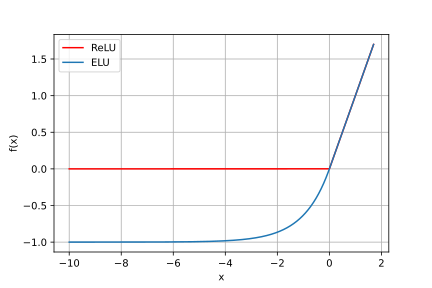
\includegraphics[width=0.5\textwidth]{figures/5_/5_relu_elu.pdf}
    \caption{Visualising the difference between the exponential linear unit (ELU) (with $\alpha = 1$) and rectified linear unit (ReLU) activation functions.}
    \label{fig:5_relu_elu}
\end{figure}

The primary reason for using ELU rather than ReLU is that one of the most significant problems of ReLU is that of \textit{dead neurons}. This problem occurs when a neuron is pushed to a negative weight (e.g. from a large update), because the gradient of the ReLU activation (its output) w.r.t the negative neuron weight will always be zero. To illustrate clearly, consider the perceptron $y = \text{ReLU}(Wx + b)$. When the a \textit{positive input} $x$ is multiplied with \textit{negative weights} $W$, the output $y$ is zero, and so too the gradient $\frac{\delta y}{\delta W}$. 
Conversely, if the \textit{input} $x$ and weights $W$ are \textit{negative}, the output $y$ is non-negative but the gradient of the output w.r.t the weights $\frac{\delta y}{\delta W} = \text{ReLU}' (x)$ is still zero because the ReLU gradient $\text{ReLU}'$ is zero for negative inputs.
As a result, the network weight will never be able to update itself as the gradient will be zero indefinitely, irrespective of the input data.
The benefit of ELU is that its gradient is non-zero for negative inputs close to zero. This helps to solve the \textit{dead-neuron problem} as it produces non-zero gradients that help to nudge network weights in the right direction, despite them having negative inputs. 

However, it can be argued that having some sparsity in the network (due to dead neurons) is actually an advantage, which is why ReLU is the default recommendation by \cite{DeepLearningBook} for modern neural networks and is also used in \cite{AMPMotionPriors} for its actor-critic MLP. Then again, too much sparsity can result in the network losing some of its generalisation capacity.

\section{Learning the Depth Representation}
\label{sec:5_learning_representation}
To tackle the unsupervised representation learning problem, we use a convolutional VAE to learn the latent representation for the depth data $\d$. We use the method presented by \cite{variational_bayes} for optimising the VAE, whose theory is outlined in \cref{subsec:2_VAE_variational_autoencoders}. Additionally, to both deal with the constrained dimension of the latent space and make our VAE suitable for collision avoidance, we introduce a custom loss function that allows us to specify which depth characteristics the VAE should prioritise in its reconstructions and choose a lightweight network architecture inspired from \cite{deepCollisionPredictorOracle}, and \cite{vae_decoder_architecture}.

\subsection{Ideal Depth Reconstruction With a Customised Reconstruction Loss}
\label{subsec:5_vae_reconstruction}
We first recall that the \textit{reconstruction loss} in \eqref{eq:2_vae_loss_estimator_single_datapoint} defines the learned behaviour of our generative network $\pdgivez$. In a vanilla VAE, it defines that the decoder $\pdgivez$ should learn to reconstruct $\d_t$ from $\z_t$, where $\z_t$ is the sampled latent code from our encoder $\qzgived$ for a given $\d_t$. Now, the key insight is that in order to properly reconstruct $\d_t$, any features of $\d_t$ that should be reconstructed must be present in $\z_t$ -- from which the VAE learned to do through the joint optimisation of the encoder and decoder in \eqref{eq:2_vae_loss_estimator_dataset}.
This implies that if we define certain features of $\d_t$ to be more costly than others, their loss will be over-represented in the reconstruction loss, and the VAE would prioritise learning these in its latent space so that these specific features could be reconstructed, and the VAE loss minimised. 

Thus, our approach is to \textit{alter the reconstruction loss} such that the VAE learns which features of the depth image distribution to prioritise in its latent space. With this, we attempt to prioritise the features in \cref{sec:4_representation_learning_task} in the latent space by presenting the following modifications:
\begin{enumerate}
    \item \textbf{Filtered targets} -- Instead of using the input $\d_t$ as the target reconstructions of our generative model $\pdgivez$, we use a filtered depth image $\d^f$ as the target. This means that for a given depth image $\d_t$, the generative network instead learns a probability distribution $\pdfgivezt$, where $\d^f_t = f(\d_t)$ is given by a deterministic filtering process $f$ of the depth image $\d_t$, and $\z_t \sim \qzgived$ is the sampled latent code from our encoder with input $\d_t$.
    \item \textbf{Depth weighting} -- We weigh the pixel-wise reconstruction error by a function of its observed depth. This means that the reconstruction error for pixels showing close obstacles in $\d^f_t$ are weighed more than pixels of far obstacles.
    \item \textbf{Added edge loss} -- We add the an additional mean-absolute error (MAE) term to the reconstruction error of filtered-obstacle edge pixels.
\end{enumerate}

To go more in detail, the filtering process is the IP-Basic algorithm \cite{filtering_depth_completion} for dilation and hole closing, as used in \cite{LearningStateRepresentation} and \cite{deepCollisionPredictorOracle}. Its implementation is a result of a few benefits for our task. First, minimising the complexity of depth images by rounding shapes emphasises only learning rough shapes. Also, as dilation increases obstacle sizes, filtering provides an extra layer of safety regarding collision avoidance. Finally, filtering also removes noise, which can be important when testing this framework on a real robotic system.
Then, to avoid the extra computational load of pre-filtering depth images on the robot, we use filtered images as reconstruction targets for some depth input, such that the VAE learns to implicitly perform the filtering process in its forward-pass \cite{LearningStateRepresentation}.

As for the depth weighting, we multiply the pixel-wise error of a reconstruction with the bounded depth gain $K_{\text{depth}}(d_{i,j})$, a function of the filtered-depth pixel value $d_{i,j}$:
\begin{equation}
    K_{\text{depth}}(d_{i,j}) = \alpha_\text{depth} \cdot \min \Bigg(\frac{1}{d_{i,j} + 0.5}, 1\Bigg) \qquad \text{for} \quad  i, j \in \dim \, (\d_t^f)
    \label{eq:5_depth_gain}
\end{equation}
which is illustrated in \cref{fig:5_depth_gain}.
\begin{figure}[hbt]
    \centering
    \includegraphics[width=0.5\textwidth]{figures/5_/5_depth_gain.pdf}
    \caption{The depth gain to weigh the pixel-wise reconstruction error. Reconstruction errors for very close obstacles (pixel values $d_{i,j}<0.16$) are weighed the same, with $\alpha_\text{depth} = 10.0$.}
    \label{fig:5_depth_gain}
\end{figure}
The idea for the depth weighting is that if we increase the reconstruction error according to its closeness, the pixel-wise loss of close obstacles should dominate the pixel-wise loss of obstacles far away. So close obstacles should be prioritised in the latent space representation.
Intuitively, this is particularly important for collision avoidance: we wish to distinguish between pixel-wise errors for obstacles far away compared to those immediately nearby. For example, a 1m error for an obstacle 7m away should be considered less important than the same as a 1m error for an obstacle 1.5m away.

We also see that thin obstacles are expected to be reconstructed when they are close by combining depth weighting with filtered targets. This is because their reconstruction targets are more prominent, as many more pixels will produce a high loss, particularly at close range.

Finally, we used a simple homemade procedure to implement the added edge loss. First, we used a Canny edge detector \cite{canny_edge_detection} to find the obstacle edges in $\d_t^f$. After, we used a Gaussian filter to dilate the edges -- taking any pixel value over 0 as an edge. Finally, the pixel-wise MAE of filtered depth reconstruction was multiplied by this image-edge mask to achieve the edge loss. Since we motivated this for clearer reconstructions, the Gaussian filter had to be used to dilate the edges of the image-edge mask. This is because, for the MAE loss to account for the object's shape, it is essential to add the pixel-wise error along the edges of obstacles and the pixel-wise error of neighbouring pixels. 


\subsection{Network Architecture}
\label{subsec:5_vae_architecture}
With the loss function covered, what remains is the architecture of the VAE. As mentioned, our VAE design was mainly inspired by the work of \cite{deepCollisionPredictorOracle} and \cite{vae_decoder_architecture}, where we utilise a convolution-based encoder-decoder structure.
The overall structure of the VAE is shown in \cref{fig:5_vae} and its parameters are detailed in \cref{app:vae_params}.
\begin{figure}[hbt]
    \centering
    \makebox[\textwidth]{
        \includegraphics[width=\textwidth]{figures/5_/5_vae.pdf}}
    \caption{The VAE network architecture. The encoder is parametrised by a CNN, while the encoder is parametrised by a transposed CNN (ConvT NN). Given a depth image $\d_t$, we can sample from the inference network $\qzgived$ to obtain a latent code $\z_t$. The generative network $\pdfgivez$ then learns to construct the filtered depth image $\d^f_t = f(\d_t)$ from the latent code$\z_t$.}
    \label{fig:5_vae}
\end{figure}

\subsubsection{Inference Network}
\label{subsubsec:5_vae_inference_network}
Our encoder is follows the CNN design of \cite{deepCollisionPredictorOracle}, though utilises instead two convolution layers before a ResNet8 \cite{KaimingResNet}, with two fully-connected layers at the end. Its structure is shown in \cref{fig:5_encoder}, while the residual blocks are depicted in \cref{fig:5_res_block}.
\begin{figure}[H]
    \centering
        \makebox[\textwidth]{
        \hspace{1mm}
        \includegraphics[width=1.\textwidth]{figures/5_/5_encoder.pdf}
    }
    \caption{The encoder network architecture. It comprises two convolution layers, with 32 $5\times5$ filters with a stride of 2, three residual blocks with $[32, 64, 128]$ output filters, and two fully connected layers with output dimensions $[128, 128]$. The dimension of the feature map is (roughly) halved for each convolution layer and residual block due to the 2-strided convolutions. The size of the feature map after the last convolution is $15\times9$. (See \cref{app:vae_encoder} for details)}
    \label{fig:5_encoder}
\end{figure}
\begin{figure}[H]
    \centering
    \includegraphics[width=0.4\textwidth]{figures/5_/5_res_block.png}
    \caption{The residual block architecture. A convolution by a $1\times1$ filter (kernel), with stride 2 is applied to the shortcut connection. $Out$ represents the number of filters of the residual block.}
    \label{fig:5_res_block}
\end{figure}
Regarding our design choices, these were primarily motivated by two factors -- we desired a lightweight network and wished to reduce the dimension of the feature map to be small enough but not too small. 
The ResNet8 was suitable to satisfy the first aspect, while the depth of the network (through stridden convolutions) was decided to satisfy the other. We also found during testing that reducing the feature dimension below $15 \times 9$ (to $8 \times 5$) resulted in a much worse reconstruction output, discouraging the use of another residual block or stridden convolution layer.
However, this choice resulted in a dramatically sized linear layer that accounted for 86\% of the encoder weights -- ($128 \cdot 15\times9) \cdot 128$ connections.
Nevertheless, this was unavoidable since 128 was the minimum number of neurons in the linear layer (64 means and log-variances), which left the alternatives: to either reduce the feature dimension or the number of filters. Though, both options were tested and did not improve results, leaving the conclusion that this is a feature and not a disadvantage of our encoder.


\subsubsection{Generative Network}
\label{subsubsec:5_vae_generative_network}
The generative network is inspired from \cite{vae_decoder_architecture}, with an additional linear layer and transposed convolution layer. Its architecture is shown in \cref{fig:5_decoder}. 
\begin{figure}[hbt]
    \centering
        \makebox[\textwidth]{
        \hspace{1mm}
        \includegraphics[width=\textwidth]{figures/5_/5_decoder.pdf}
    }
    \caption{The decoder network architecture comprises two linear layers and seven transposed convolution layers. Each strode transposed convolution roughly the dimension of the feature map to achieve the final dimension feature map dimension $480\times270$. (See \cref{app:vae_decoder} for details)}
    \label{fig:5_decoder}
\end{figure}
The primary design rule for autoencoders is that the decoder should be a mirror of the encoder so that the network resembles an \textit{hourglass}. As a result, we followed the encoder with two linear layers, including the large linear layer that connects 128 neurons to 128, $9\times5$ filters. As for the transposed convolutions, this is a relatively simple but effective design. The only design choice here was the filter size and number of filters, though these were chosen primarily to match the layer-wise feature dimensions of the encoder and their overall sizes.

Vigorous testing was also done with a ResNet8 decoder, which was designed to mirror our encoder. However, despite its more advanced structure -- with batch normalisation and shortcut connections -- no significant performance gain was observed in training. Conversely, checkerboard artefacts and divergence in training were often observed when training on the whole dataset due to uncertain reasons, though it could be to the layer-wise stacking of stridden transposed convolutions with identical filter dimensions \cite{odena2016deconvolution}. Therefore, a final decision was made to use the decoder in \cref{fig:5_decoder}.
\chapter{Implementation}
\label{chap:6_implementation}

In this chapter, we will present the implementation details and software frameworks used in this thesis.
First, we describe the training setup for the VAE and the MLP. This will include the procedure for collecting a depth images dataset for VAE training, and how we define our quadrotor task in the Isaac Gym framework. Finally, we present how we define our CNN-MLP model using a reinforcement learning library, \textit{RL Games} \cite{rl-games2022}, and discuss some details of the PPO implementation.

\section{Collecting a Filtered Dataset of Depth Images}
To collect the depth for VAE training, we used a pre-existing simulator that had been developed in \cite{deepCollisionPredictorOracle}. This is the RotorS \cite{RotorS_Furrer2016} simulator, which is an extension to the simulation framework, Gazebo \cite{Gazebo}. Here, Gazebo is a is an open-source physics-based robotics simulator that allows us to design and test custom robotic models. RotorS is then a quadrotor simulator that builds on this, providing a variety of packages that range from quadrotor models to controllers to sensors. 

To use RotorS for their task, \cite{deepCollisionPredictorOracle} added a quadrotor model resembling their real-life resilient micro-flyer (RMF) to RotorS, equipped with a simulated depth camera with the same specifications as an Intel RealSense Depth Camera D455, with resolution $480 \times 270$. Then to generate a dataset, the quadrotor was flown with random velocities and steering angles in a randomised environment in Gazebo until collision. While \cite{deepCollisionPredictorOracle} was interested in the state-action-collision labelled dataset, we used this framework to simply collect the depth images.

Then, since we are only interested in the depth images, we flip these along their vertical axis to double the total. With almost 400,000 depth images, we filtered each of these with the IP-basic algorithm \cite{filtering_depth_completion} and batched them into TensorFlow Record files. Finally, we wrapped the record files in a PyTorch Iterable Dataset to ensure that not all depth images would be loaded into memory when iterating through the dataset.



\section{Quadrotor Task in Isaac Gym}
We utilise \textit{Isaac Gym} \cite{IsaacGym} as a large-scale parallel hardware-accelerated (GPU) simulator to initialise and run 512 environments simultaneously. Through its end-to-end GPU simulation, it avoids performance bottlenecks in CPU-GPU data transfers and allows for a high performance and simulation throughput on a single GPU.

To use Isaac Gym for our task, we first have to define an MDP-like \textit{quadrotor task} that we can perform reinforcement learning in -- similar to any standard gym environment in OpenAI Gym \cite{openAIgym}. Essentially, we have to create a quadrotor model, then define its states, actions, the state-transition dynamics and the rewards an agent receives per state-action timestep. Fortunately for us, there was related task, namely \textit{Quadcopter} example in Isaac Gym, that we could adapt to our task. From this, we could use the existing quadrotor model and its states, but just redefine its observation and action spaces, the reward function and environment.

\subsection{Agent}
Beginning first with the agent, we wished to have an observation space $S_t = [\s_t, \d_t]$ consisting of the quadrotor state and depth images. To obtain the depth images, Isaac Gym allows us to add camera sensors with specific properties. Choosing its properties to model the same depth camera used to collect the VAE images, we then attached the camera to the quadrotor body using Isaac Gym's API with a follow transform to obtain depth images $\d_t$ in simulation.

As for state of the agent $\s_t$, Isaac Gym's API allows us to obtain the states of all \textit{actors} (Isaac Gym assets) through a \textit{root tensor}, where every state contains 13 floats, matching \eqref{eq:4_quadrotor_states}: 3 floats for position, 4 for quaternion, 3 for linear velocity, and 3 for angular velocity. By indexing the quadrotor asset, we could then access the true quadrotor state at every time step.

As for the action space, Isaac Gym allows us to control an \textit{actor} by specifying its motion directly or through its control tensors, such as applying forces to a robot's degrees of freedom. Though not recommended, we opted for the first option due to simplicity -- simply altering the quadrotor state in the root tensor to be the desired action velocity and yaw rate. This is of course non-physical behaviour since we override Isaac Gym's physics engine, meaning that changes in velocities would be instantaneous. 
To provide some compensation for this, we adjusted the simulation timestep to be \textit{dt} $= 0.2$ seconds, which ensures that there is a suitable bandwidth separation between the reinforcement learning agent “action frequency” and an eventual closed-loop control system bandwidth, so that we can expect that an underlying control system has time to set $\v_t = \v_t^d$ at each timestep. Nonetheless, since our thesis aims to demonstrate motion planning, this choice was thought to be reasonable (given the time constraints).

\subsection{Environment}
With the agent ready, we now had to define the environment that the quadrotor was to operate in. The obstacles used in this thesis were loaded as Isaac Gym assets through Unified Robotic Description Format (URDF) files. Most importantly, these described the visual and collision geometry of various shapes, including our quadrotor model and goal. 
In Figures \ref{fig:6_quad_goal} and \ref{fig:6_obstacles} we show the quadrotor, goal and added obstacles to our environment.
\begin{figure}[H]
     \centering
     \hspace{0.04\textwidth}
     \begin{subfigure}[b]{0.3\textwidth}
         \centering
         \captionsetup{justification=centering}
         \includegraphics[width=\textwidth]{figures/6_/6_quadrotor.png}
         \caption{Quadrotor}
         \label{fig:6_quadrotor}
     \end{subfigure} 
     \hspace{0.15\textwidth}
     \begin{subfigure}[b]{0.32\textwidth}
         \centering
         \captionsetup{justification=centering}
         \includegraphics[width=\textwidth]{figures/6_/6_goal.png}
         \caption{Goal}
         \label{fig:6_goal}
     \end{subfigure} 
     \caption{Quadrotor and goal assets in our Isaac Gym environment. These are both standard assets already present in Isaac Gym, and are borrowed for this task. The quadrotor does not collide with the goal, nor is the goal visible in the depth images.}
     \label{fig:6_quad_goal}
\end{figure}

With defined collision geometries, we could then enable collisions in the environments by placing obstacles in the same environment in the same collision group, and setting their collision filters to be 1. Since we do not want collisions with the goal however, we simply removed its collision geometry -- rendering it invisible to the depth camera and the possibility for collision. The collision filter was also set to 0, but this made did not remove it from depth images.

Finally, to place these obstacles nicely in our environment, we could change the object dimensions in the URDF files, and do further scaling of objects in Isaac Gym. Then, through the root tensor, we were able to adjust their poses through rotations and randomise their position.

\begin{figure}[H]
     \centering
     \hspace{0.04\textwidth}
     \begin{subfigure}[b]{0.3\textwidth}
         \centering
         \captionsetup{justification=centering}
         \includegraphics[width=\textwidth]{figures/6_/fence.png}
         \caption{Fence}
         \label{fig:6_obst_fence}
     \end{subfigure} 
     \hspace{0.15\textwidth}
     \begin{subfigure}[b]{0.3\textwidth}
         \centering
         \captionsetup{justification=centering}
         \includegraphics[width=\textwidth]{figures/6_/pine_tree.png}
         \caption{Pine tree}
         \label{fig:6_obst_pine_tree}
     \end{subfigure} 
     \hfill \\[2mm]
     \hspace{0.04\textwidth}
     \begin{subfigure}[b]{0.3\textwidth}
         \centering
         \captionsetup{justification=centering}
         \includegraphics[width=\textwidth]{figures/6_/simple_u.png}
         \caption{Simple U-shape}
         \label{fig:6_obst_simple_u}
     \end{subfigure} 
     \hspace{0.15\textwidth}
     \begin{subfigure}[b]{0.3\textwidth}
         \centering
         \captionsetup{justification=centering}
         \includegraphics[width=\textwidth]{figures/6_/chair.png}
         \caption{Chair}
         \label{fig:6_obst_chair}
     \end{subfigure}
     \hfill \\[2mm]
     \hspace{0.04\textwidth}
     \begin{subfigure}[b]{0.3\textwidth}
         \centering
         \captionsetup{justification=centering}
         \includegraphics[width=\textwidth]{figures/6_/simple_stone.png}
         \caption{Simple stone}
         \label{fig:6_obst_simple_stone}
     \end{subfigure} 
     \hspace{0.15\textwidth}
     \begin{subfigure}[b]{0.3\textwidth}
         \centering
         \captionsetup{justification=centering}
         \includegraphics[width=\textwidth]{figures/6_/simple_pyramid.png}
         \caption{Simple pyramid}
         \label{fig:6_obst_simple_pyramid}
     \end{subfigure} 
    \caption{Various obstacles are imported to our Isaac Gym environment through their URDF files. Their defined collision geometries allows them to be visible in the depth images and allows the physics engine to simulate collisions with them. By altering their dimensions and \textit{root tensors}, we could fit them nicely in our environments, with randomised poses.}
     \label{fig:6_obstacles}
\end{figure}

\newpage
\subsection{Parallel Initialisation}
In regards to the parallel initialisation of the environments, this is dependent on which stage of the curriculum we are training on.
In the first scenario with no obstacles, we initialise each environment to have a quadrotor and goal with random positions in an area $x, y \in [-3, 3]$, with $z \in [-0.2, 2]$. Furthermore, we add a ground plane at $z = 0$, and mimic ``far obstacles'' by confining each quadrotor to a $16\times8$ enclosure. This serves to bias the agent to initially ignore the depth representation input while it learns to map the quadrotor states to correct actions. 

Then, for 1-obstacle environments, the quadrotor and goal for each environment is now placed at each end of their enclosure, with an obstacle placed in the middle. Their initialised $x$ positions are fixed (along the long axis), but are randomised in $y$ (short axis). Also, the quadrotors and goals are also slightly randomised in $z$. Then, we extend this design to $n$-obstacle environments, where we gradually increase the environment size and number of obstacles in between a quadrotor and goal, but ensuring that a quadrotor always has $3$m of open space before the first obstacle. An example is shown in \cref{fig:6_n_obst_env}.
\begin{figure}[hbt]
    \begin{subfigure}[b]{0.69\textwidth}
        \centering
        \includegraphics[width=0.99\textwidth]{figures/6_/6_environments.png}
        \caption{512 environments are initialisation in parallel.\vspace{8mm}}
        \label{fig:6_environments}
    \end{subfigure}
    \hfill
    \begin{subfigure}[b]{0.3\textwidth}
        \centering
        \includegraphics[width=0.7\textwidth]{figures/6_/6_n_obst_env.png}
        \caption{Quadrotor, goal and obstacle positions are randomised in $y$ for each environment.}
        \label{fig:6_n_obst_env}
    \end{subfigure}
    \caption{An example of the parallel initialisation of environments and their obstacle placements with Isaac Gym \cite{IsaacGym}. We simulate 512 environments in parallel, where the quadrotor and goal is initialised at each end of a corridor-like enclosure with obstacles placed in between. Positions of each item are fixed in the $x$ (long axis), but randomised in $y$ (short axis). Quadrotor and goal heights (in $z$) are also slightly randomised.}
    \label{fig:6_env_init}
\end{figure}


\section{Model Implementation and PPO in RL Games}
Now that the reinforcement learning framework was prepared, we used a reinforcement learning library called \textit{RL Games} \cite{rl-games2022} to implement our CNN-MLP network to be trained with PPO.
The RL Games integration with IsaacGym follows strictly hierarchical structure where all specific algorithms and models inherit from general base implementations. In this way, the training setup is defined through configuration files managed by \textit{Hydra}\footnote{See how IsaacGymEnvs uses Hydra at: \url{https://github.com/NVIDIA-Omniverse/IsaacGymEnvs}.}. 

\subsection{Implementing our Model}
To integrate our model with RL games, we identified that main challenge is not how to implement PPO with our model, but how to integrate our custom network into RL Games. If we could solve this, we could then specify that our model should use our custom network in configuration, and this should allow it to be seamless optimised with PPO.
So to solve this, we first wrapped our custom network in a \textit{network builder}. From here, we could use the \textit{model builder} to register our network in RL Games' network registry during initialisation. As a result, our network was now a part of RL games and could be chosen as for any reinforcement learning task.

Then, to use it in our custom quadrotor task, we define two configuration files, one for the setup of the quadrotor task and the other to define the model. Here, the task configuration is quite standardised, including the dimension of observation and action space, simulation parameters like $dt$, but also the number of obstacles, environment size and episode length. In contrast, the training file provided our model definition, consisting of the optimisation algorithm and its hyperparameters (batch size, learning rate, trajectory length, etc.), and our network and its hyperparameters (size, activation functions, normalised actions, separate actor-critic networks, etc.).

\subsection{Normalised and Clipped Observation and Action Space}
Next, there are some noteworthy details of the our model implementation that is relevant for our task. The first is that normalising the observation and action spaces is of particular importance in RL Games, first introduced in \cite{DDPG} and iterated also in the documentation of Stable-Baselines3, ``normalising input features may be essential to successful training of an RL agent'' \cite{stable-baselines3}. \textit{Normalising} can mean two different things in reinforcement learning, either by scaling observations to $[0, 1]$ or to have 0 mean and 1 standard deviation. The perspective this thesis takes is that image values are scaled, while everything else is normalised.
So, to normalise the observation space in our quadrotor task, we begin by scaling our images and quadrotor states by a function of their max values. The idea is that when we gradually increase the environment size to larger values, i.e. greater $\p_t$ from goal, this should not alter the policy performance. Later, the scaled quadrotor states (and not the depth image) is then normalised its running mean and covariance, whose values are calculated throughout the training process.
For the actions, these are not normalised but instead clipped if their values exceed 1, which was also why we avoided using a non-linear activation function for our actor-critic. For good measure, the observations space is also clipped to a max value of 5 before being normalised by its running mean and standard deviation.

\subsection{Experience and Optimisation}
In order to perform optimisation, PPO requires that data (experience) is sampled by its current policy into a trajectory $\boldsymbol{T}$, where each \textit{experience} element is given by a tuple $<S_t, A_t, R_t, S_{t+1}$. In the parallel learning scheme, observations $S_t = [\s_t, \d_t]$ from each environment is compiled into an observation buffer $O_t$ for each time timestep. As mentioned, these observations are then clipped and normalised, before being sent to the actor to provide actions for the current policy $\pi$. Though we simulate 512 environments, there is only one network -- for each timestep, we batch the 512 observations into an input tensor of $[512, 129613]$ and compute the forward-pass for the whole batch. The batched depth images are sent separately to the to the VAE, such that we receive $[512, 64]$. Then, by concatenating it with the quadrotor state tensor to get $[512, 64]$, our actor-critic outputs a batched action tensor $[512, 3]$. Finally, our agent observes rewards $[512, 1]$ to which it can compare to its value estimate to calculate the advantage estimate.

Throughout this process, an \textit{experience buffer} collects the state-action pairs as the trajectory. We define the \textit{horizon} or \textit{trajectory length} to be $T=8$, such that our batch size is $512\cdot8 = 4096$. We also define a minibatch size of $M=1024$ and number of mini-epochs $K=8$. Overall, we first simulate our environment in parallel for 8 timesteps to collect a trajectory. With this we optimise for our PPO loss in minibatches, and repeat the optimisation on the trajectory for $K=8$ mini-epochs. Finally, we discard the trajectory and run the simulation for 8 timesteps to collect a new trajectory, and so on. Lastly, when calculating the gradients for the trajectory, we also utilise truncated gradients where the gradients are scaled according to Pytorch's \textit{GradScaler} and clipped by their norm.



\chapter{Navigation Policy Evaluation Studies}
\label{chap:7_navigation_policy_evaluation_studies}

In this chapter, we present and evaluate our approach in developing an efficient collision-free navigation policy. Our approach is presented in the context of the curriculum, where we share the step-by-step decisions and thought process for training our policy.
The final policy is then evaluated, where we assess its performance in its training environment and its ability to generalise to new environments.

For our thesis, training and simulation was done on an Intel(R) Core(TM) i9-10940X CPU @ 3.30GHz desktop PC, with a NVIDIA GeForce RTX 3090 GPU. 

\section{Policy Performance along the Learning Curriculum}
\label{sec:7_learning_curriculum}
In this section, we analyse the training characteristics of our navigation policy in progressively difficult environments. In total, our curriculum is composed of 7 levels, with an initial pretraining stage. An overview of the training time and environment setup is shown in Figures \ref{tab:7_curriculum} and
\ref{tab:7_curriculum_space} respectively.
\begin{table}[hbt]
    \centering
    \begin{tabular}{||c|c|c|c||}
    \hline
    Level & No. of Obstacles & Iterations & Time \\
    \hline\hline
    0 & 0 - Pretraining & 97 & 12m \\ \hline
    1 & 0 & 95 & 11m \\ \hline
    2 & 1 & 808 & 1h 40m \\ \hline
    3 & 3 & 652 & 1h 22m \\ \hline
    4 & 5 & 1498 & 3h 12m \\ \hline
    5 & 9 & 3500 & 7h 38m \\ \hline
    \end{tabular}
    \caption{The learning curriculum for the navigation policy. The total time for training is all seven policies is 14h 15m, with 6650 total iterations. One iteration is given by the length of the trajectory $\boldsymbol{T}$, defined as 8 simulation timesteps.}
    \label{tab:7_curriculum}
\end{table}
\begin{table}[hbt]
    \centering
    \begin{tabular}{||c|c|c|c|c||}
    \hline
    Level & No. of obstacles & Env. Size & Obst. Area & Space per obst. \\  & & & & (m$^2$ / obst.) \\\hline\hline
    0 \& 1 & 0 & 16, 8 & - & - \\\hline
    2 & 1 & 16, 8 & 32 & 32.0 \\\hline
    3 & 3 & 20, 10 & 80 & 26.67 \\\hline
    4 & 5 & 20, 10 & 80 & 16.0 \\\hline
    5 & 9 & 20, 10 & 80 & 8.89 \\\hline
    \end{tabular}
    \caption{Environments used in the curriculum. We specify the ``openness'' per environment as a more intuitive measure for clutter rather than obstacle density. The obstacle area begins 6m from each end of the enclosure to allow space for the quadrotor and goal. Thus, the obstacle area is given by $A = (X - 12) \cdot Y$.}
    \label{tab:7_curriculum_space}
\end{table}
For each environment, the policy performance will be briefly analysed in the context of \textit{average return} across all environments and the \textit{episode end information} for the last 1000 episode ends.

\subsubsection{Understanding the Average Return and End Info Plots}
The average return in this case is given by the average accumulated rewards across all environments, giving an indication of the overall navigational efficiency of the robot as the reward function is centered around the quadrotor reaching its goal. 
However, to ensure that robots are constantly exploring the environment dynamics and learning collision avoidance, we specify an end episode timestep $T$ that resets the environment and places the quadrotor back to its initial position. This significantly changes the average rewards in the scenario that multiple environments are reset, producing sharp drops or spikes in the average return plots.

Since the reward is centered around reaching goal, there is a good chance that the learned policy is not exactly ideal in terms of collision avoidance. Thus, we include the the episode end label as an abstract continuous indicator of the collision rate for the current policy. We can expect that if both the collision rate and average return is high, the quadrotor is quite aggressive in flying towards goal, sacrificing some collisions in order to exploit high rewards near goal. In contrast, if both are low, we can imagine that the policy does not have an idea of how to exploit the reward system but avoids collisions, meaning it is overly conservative and does not reach the goal, despite not crashing. In the extreme case where the reward is very low and the collision rate is high, this suggests that the policy has \textit{diverged} -- i.e. the weights of the network are so far from its optimal configuration space that it is unable to perform meaningful actions. Most clearly, the desired policy is opposite of this: with maximum return and minimal collision. 
In addition, since the end information is averaged over 1000 episodes, there is a small \textit{delay} when observing the collision avoidance properties from a current policy. As a result, the policies that are collision avoidant should either have positive slopes for timeout-episodes or maintain its low collision rates for subsequent episode ends. 

Finally, we specify bounds on the quadrotor height, where the quadrotor is reset if $z$-position goes beyond $[0, 3]$. Hence, there are three ways an episode can end: through this \textit{out of bounds} in $z$, through \textit{timeout} after $T$ timesteps, or \textit{collisions} where an obstacle is $<0.2m$ away from it or there is contact on the sides.
 
\subsection{Without Obstacles}
\begin{figure}[H]
    \centering
    \begin{subfigure}[b]{\textwidth}
        \centering
        \captionsetup{justification=centering}
        \includegraphics[width=0.99\textwidth]{figures/7_/3DCarModel_BodyObs_0_NewObs_v0_reward.pdf}
        \label{fig:0_obst_pretraining_rew}
    \end{subfigure} \\
    \begin{subfigure}[b]{\textwidth}
        \centering
        \captionsetup{justification=centering}
        \includegraphics[width=0.99\textwidth]{figures/7_/3DCarModel_BodyObs_0_NewObs_v0_end_info.pdf}
        \label{fig:0_obst_pretraining_end}
    \end{subfigure} 
    \caption{Initialising the navigation policy. The quadrotor and goal is randomly initialised in a $[-3,3]$ area with heights $z \in [0.2, 2.0]$. The best model is selected at 97 iterations.}
    \label{fig:7_train_pretraining_no_obst}
\end{figure}
As stated in \cref{subsec:5_curriculum}, before a quadrotor learns collision avoidance, it must first learn to fly towards a goal. Given that our observation-action mapping space is quite large ($\R^{77} \rightarrow \R^{3}$), our initial guess was that navigating towards a waypoint could already be quite challenging given that we are in the continuous domain. 
With this expectation, we trained our policy with results in \cref{fig:7_train_pretraining_no_obst}.
From this figure, we can observe that pretraining is very successful, where the quadrotor steadily increases its average return at the same time its collision rate drops. By just 30 iterations (4 minutes), we see that the agent reaches its goal 100\% of the time and maximises its potential reward for most of the episode.

The next step taken is to initialise the quadrotor and goal in its new environment setup, where each are placed at the end of the environment. This is a relatively simple training stage that we expect should be completed with ease. 
\begin{figure}[htb]
    \centering
    \begin{subfigure}[b]{\textwidth}
        \centering
        \captionsetup{justification=centering}
        \includegraphics[width=0.99\textwidth]{figures/7_/3DCarModel_BodyObs_NavSetup_0_NewObs_v0_reward.pdf}
        \label{fig:0_obst_nav_rew}
    \end{subfigure} \\
    \begin{subfigure}[b]{\textwidth}
        \centering
        \captionsetup{justification=centering}
        \includegraphics[width=0.99\textwidth]{figures/7_/3DCarModel_BodyObs_NavSetup_0_NewObs_v0_end_info.pdf}
        \label{fig:0_obst_nav_end}
    \end{subfigure}
    \caption{Conditioning the policy to its new state distribution. The best model is selected at 95 iterations.}
    \label{fig:7_train_nav_no_obst}
\end{figure}
From \cref{fig:7_train_nav_no_obst}, we see that this is true, where we mostly observe timeouts.

\subsection{1 Obstacle}
\label{subsec:7_1_obstacle}
Before the first obstacle is added, the agent does not necessarily have to learn to avoid close obstacles. In this situation however, obstacles are placed directly in between the quadrotor and goal, such that to achieve a low collision rate, some degree of collision avoidance is necessary.
\begin{figure}[htb]
    \centering
    \begin{subfigure}[b]{\textwidth}
        \centering
        \captionsetup{justification=centering}
        \includegraphics[width=0.99\textwidth]{figures/7_/3DCarModel_BodyObs_NavSetup_1_NewObs_v1_reward.pdf}
        \label{fig:1_obst_nav_rew}
    \end{subfigure} \\
    \begin{subfigure}[b]{\textwidth}
        \centering
        \captionsetup{justification=centering}
        \includegraphics[width=0.99\textwidth]{figures/7_/3DCarModel_BodyObs_NavSetup_1_NewObs_v1_end_info.pdf}
        \label{fig:1_obst_nav_end}
    \end{subfigure} 
    \caption{Training with 1 obstacle. The best model is selected at 808 iterations, with an average return of 422 and timeout rate of $95.6\%$.}
    \label{fig:7_train_nav_1_obst}
\end{figure}
Despite this new challenge, we see that the quadrotor does well to cope -- steadily decreasing its collision rate to about 4\% in about 160 iterations (20 minutes), and to a minimum of about 2\% at 600 iterations. Though, in regards to policy performance, we note that the average return follows a very oscillatory behaviour which is reflected very slightly in the collision rate. Intuitively, this can be explained by the agent exploring its state-space, which consequently can be good or bad -- the quadrotor cannot know that colliding with an obstacle always leads to a negative reward until it has experienced it repeatedly from various positions. 
However, since we did surround the quadrotor in a rectangular enclosure, it was observed that the quadrotor managed to learn to not crash into walls quite early, albeit to a small degree. Just by simply stopping and turning though, is enough to pass this level.

We observe that it is not until the third oscillation in the average return that the agent finds an optimal policy which combines high total rewards with low collision rates. After this, we do observe that the collision probability falls even lower, but so too does the reward gained. Thus, we remind ourselves that we want \textit{both} navigational efficiency and conservativeness in our policy. For this training stage, we selected the model at 808, which had a good combination of both.

An early behaviour that was also observed during training is that the quadrotor learned to pick a ``favourite side'' when avoiding obstacles -- sometimes it always passed on the left, other times always on the right, despite it being more open on the other side. To try and explain this, we have to remember that neural networks are function approximators. In some sense, we can think of ``seeing the obstacle'' as a variable that is sometimes positive (or zero) in the latent code. If it is not there, we go straight, but if it is there, we turn to one side -- deterministically. We can imagine that if the agent is directly in front and in the middle of an obstacle, unless the policy is randomised to a significant extent, the same values in the input should result in the same action.

\subsection{3 Obstacles}
\label{subsec:7_3_obstacles}
Continuing onwards to three obstacles, we expect that similar to one obstacle, we should observe oscillations in the return as the agent explores different approaches to solving the navigation task. We also expect that since the obstacle has learned how to avoid one obstacle, it should be be straightforward to generalise this to three -- particularly when the objects are placed far apart.
\begin{figure}[htb]
    \centering
    \begin{subfigure}[b]{\textwidth}
        \centering
        \captionsetup{justification=centering}
        \includegraphics[width=0.99\textwidth]{figures/7_/3DCarModel_BodyObs_NavSetup_3_NewObs_v1_reward.pdf}
        \label{fig:3_obst_nav_rew}
    \end{subfigure} \\
    \begin{subfigure}[b]{\textwidth}
        \centering
        \captionsetup{justification=centering}
        \includegraphics[width=0.99\textwidth]{figures/7_/3DCarModel_BodyObs_NavSetup_3_NewObs_v1_end_info.pdf}
        \label{fig:3_obst_nav_end}
    \end{subfigure} 
    \caption{Training with 3 obstacles. The best model is selected at 652 iterations, with an average return of 514 and timeout rate of $89.7\%$.} %1652
    \label{fig:7_train_nav_3_obst}
\end{figure}
From \cref{fig:7_train_nav_3_obst}, we see that these expectations are largely matched -- with the average accumulated reward varying significantly and the collision rates steadily increasing. From this, we observe that the a good combination of both is just about in between 600 and 700 iterations, such that we choose the best model at 652 iterations.

One of the most pertinent differences that we can observe in this scenario is that the highest timeout rates are consistently lower than before. We can accept that since the agent is essentially re-learning a more complex state-action mapping -- e.g. meeting obstacles at the edge of the environment after turning -- we do not expect high timeout rates immediately. Yet, eventually, we do expect that if it can reach the goal $>95\%$ of the time for 1-obstacle environments, it should be able to do the same here, given a similar ``optimal'' policy. 
However, this reasoning is slightly unfair since the agent now has to perform three times more collision-free manoeuvres than in the previous case. Thus, if the agent can manoeuvre past one obstacle with $95\%$ success, it is only fair to assume for a success rate of $95\%^3 \sim 85\%$ for the three obstacle environment.
From this perspective, we then see that the policy is improving, since it does achieve over an over $90\%$ timeout rate at its best point. 

\subsection{5 Obstacles}
\label{subsec:7_5_obstacles}
When approaching more cluttered environments, an effective navigation policy has to learn to carefully judge actions as a function of more than one visible obstacles. It cannot simply navigate to one side of an obstacle, but base the extent and direction of its turns from what it sees. This is a natural consideration that even takes time learn, even for humans. 
We thus expect that policy learning will progressively take longer in more complex environments as the agent learns to fine-tune this behaviour. Based on this assumption, we train the policy for significantly longer ($\approx 6800$ iterations) and increase the end episode timestep $T$ to compensate for manoeuvring time. The result of which is shown in \cref{fig:7_train_nav_5_obst}.
\begin{figure}[htb]
    \centering
    \begin{subfigure}[b]{\textwidth}
        \centering
        \captionsetup{justification=centering}
        \includegraphics[width=0.99\textwidth]{figures/7_/3DCarModel_BodyObs_NavSetup_5_NewObs_v1_reward.pdf}
        \label{fig:5_obst_nav_rew}
    \end{subfigure} \\
    \begin{subfigure}[b]{\textwidth}
        \centering
        \captionsetup{justification=centering}
        \includegraphics[width=0.99\textwidth]{figures/7_/3DCarModel_BodyObs_NavSetup_5_NewObs_v1_end_info.pdf}
        \label{fig:5_obst_nav_end}
    \end{subfigure} 
    \caption{Training with 5 obstacles. The best model is selected at 1498 iterations, with an average return of 720 and timeout rate of $94.8\%$.} %3150
    \label{fig:7_train_nav_5_obst}
\end{figure}
Once again, we observe from the figure a similar pattern for the return in the first 1000 iterations. However, unlike the 3-obstacle case, we recognise that the environment is indeed more difficult, resulting in a more complex optimisation space that causes higher fluctuations in the accumulated rewards when the agent explores different trajectories. This is also more pronounced due to the longer episode times, such that if a policy does well to reach the goal it will accumulate significantly more rewards than one that does decent but does not reach goal as closely or as often.

Another promising feature of this training plot is that the timeout rates are consistently higher than for the 3-obstacle case, even when the reward is high. The reason for this is quite indirect, though will be discussed later in \cref{subsec:9_sparse_rewards}.
Keeping this optimistic perspective, we can then move on to 9-obstacles.


\subsection{9 Obstacles}
\label{subsec:7_9_obstacles}
The most difficult environment of the training process consists of 9 obstacles in an $20\times10$ environment. Accounting for the quadrotor and goal -- a 6m spacing as seen in  -- the effective area for this obstacles is an $8\times10$ square, or an obstacle every metre for 8m. 
For perspective, we provide two images in \cref{fig:7_9_obst_and_flat_png}. 
\begin{figure}[htb]
    \centering
    \begin{subfigure}[b]{0.26\textwidth}
        \centering
        \captionsetup{justification=centering}
        \includegraphics[width=0.99\textwidth]{figures/7_/7_9_obst.png}
        \caption{9 obstacles are placed from along $x \in [-4,4]$.}
        \label{fig:9_obst_png}
    \end{subfigure}
    \hfill
    \begin{subfigure}[b]{0.71\textwidth}
        \centering
        \captionsetup{justification=centering}
        \includegraphics[width=0.99\textwidth]{figures/7_/7_9_obst_flat.png}
        \caption{Agent must display collision avoidant properties to pass.}
        \label{fig:9_obst_flat_png}
    \end{subfigure} 
    \caption{An example environment with 9 obstacles, with size $20\times10$.}
    \label{fig:7_9_obst_and_flat_png}
\end{figure}

Following the same idea for the 5 obstacle case, we provided ample time for policy training and kept the episode length $T$ the same to obtain the results in  \cref{fig:7_train_nav_9_obst}.
\begin{figure}[htb]
    \centering
    \begin{subfigure}[b]{\textwidth}
        \centering
        \captionsetup{justification=centering}
        \includegraphics[width=0.99\textwidth]{figures/7_/3DCarModel_BodyObs_NavSetup_9_NewObs_EnvSpace10_last3150_v1_reward.pdf}
        \label{fig:9_obst_nav_rew}
    \end{subfigure} \\
    \begin{subfigure}[b]{\textwidth}
        \centering
        \captionsetup{justification=centering}
        \includegraphics[width=0.99\textwidth]{figures/7_/3DCarModel_BodyObs_NavSetup_9_NewObs_EnvSpace10_last3150_v1_end_info.pdf}
        \label{fig:9_obst_nav_end}
    \end{subfigure} 
    \caption{Training with 9 obstacle. The best model is selected at 3500 iterations, with an average return of 700 and timeout rate of $84.7\%$. }
    \label{fig:7_train_nav_9_obst}
\end{figure}
Here, we see that the average return follows an upwards trend to about 1500 iterations, which reflects the difficulty of the environment as the agent takes much longer time to fine-tune its behaviour. Interestingly, we see that this trend also applies to the timeout rate but only to about 1000 iterations. This suggests that the rewards for collision avoidance and goal-reaching are aligned up some degree, but at some point, the rewards motivate the agent to learn risky behaviour -- prioritising to reach goal in situations where it could be more careful.

However, after extensive sampling, we see that the agent policy begins to learn very promising collision avoidance attributes between iterations $3200 \sim 3600$, where we select our best model at 3500 iterations. In this situation, we also note that the average return varies dramatically. To reason for this, we can assume that when the agent is learning to navigate carefully, i.e. the policy is aware of state-actions pairs that cause collisions, the conservative behaviour could mean reaching goal is unlikely. This is in contrast to the policy at around 1500 iterations which learned to ``consistently'' reach goal, though ironically with crashes. So in our situation, we can view the model at $3500$ iterations as having a good balance of both, where the policy has ``stumbled upon'' a favourable locally optimal solution with good navigational abilities.

The reason that conservative policies have a hard time reaching goals is also linked to the observation that collision rates are relatively high. Unfortunately, this is expected, and can be explained by the agent having to manoeuvre past more obstacles in the previous case. Moreover, due to the more cluttered nature of the environment, the agent can also experience \textit{getting stuck} in between obstacles where there is no clear way forward.
An example of this is shown in \cref{fig:7_9_obst_and_flat_png}, where we see a corner-type situation of the left side in between the tree and U-shape, and can observe a quadrotor flying. Of course, we can think that a quadrotor getting stuck in this situation is unlikely, seeing that it could go right for example. Yet, with 512 randomly generated environments, we can imagine that these corner-type situations could exist in many forms, both on the left and right side. We can also argue that after passing an obstacle on the left, the optimal path may be to turn and look to the right, but the quadrotor will not see this due to a limited field-of-view ($86\degree$) of the camera sensor. As a result, it will enter a corner situation, (and possibly pass) as the agent shown in \cref{fig:9_obst_flat_png}. 

So, from this corner situation, if the policy is conservative, an agent will lie and wait as to avoid collision. If it is more aggressive, it will enter and risk collision. Thus, on average, a policy that remains stuck in these unlikely situations will gather much less return that one that collides, and proceeds to find the goal in the next episode -- which provides an explanation to why higher timeout rates does not equal higher rewards. However, by chance, a policy that is both conservative \textit{and} can escape corner situations could appear, which is the case for our policy at 3500 iterations shown in \cref{fig:9_obst_flat_png}.


\section{Evaluating the Learned Navigation Policy}
\label{sec:7_evaluating_policy}

With a policy selected from the curriculum, we can now evaluate its performance in the form of standardised tests in known and unknown environments, along with assessing its robustness to noise.
For the known environments, we aim to present three variations of the environment with an increasing degree of clutter, while for unknown environments we increase the environment size.
From this, we should be able to gauge its overall performance and more interestingly its ability to generalise to unseen domains and uncertainty.

\subsection{Known Environments}
For the known environments, we test the agent in an environment of size $[20, 10]$, where we increase the number of obstacles from 7 to 12, as shown in \cref{tab:7_known_tests}. Unlike training, we use a non-randomised environment such that we can visualise the behaviour of different policies in a standardised context. We then run our policy in each environment for 1000 episodes and document the episode end label.
\begin{table}[htb]
    \centering
    \begin{tabular}{||c|c|c|c|c|c|c||}
    \hline
    Level & No. of & Space per obst. & Timeouts & Collisions & Out. of & Timeout \\  
     & obstacles & (m$^2$ / obst.) & & & bounds & rate (\%) \\\hline\hline
    Easy    & 7  & 11.4   & 980 & 21 & 0 &  97.9 \\\hline
    Medium  & 9  & 8.89   & 967 & 33 & 2 &  96.5 \\\hline
    Hard    & 12  & 6.67  & 771 & 230 & 0 & 77.0 \\\hline
    \end{tabular}
    \caption{For the known environments, we evaluate the agent's response to a variation in the cluttered-ness of the environment. We choose an environment size of $[20, 10]$, which is an $8\times 10$ or 80m$^2$ effective obstacle area.}
    \label{tab:7_known_tests}
\end{table}

From the table, it is clear that the reinforcement learning agent is extremely successful in navigating \textit{known} cluttered environments, though its performance is bounded by the available space to some extent. Compared to our expectations from training, these are certainly impressive results, given that the timeout rate for the 9-obstacle environment is 96.5\% timeout rate compared to $84.7\%$ in \cref{fig:7_train_nav_9_obst}. An explanation for why we did not see such a high timeout rate in training is because the end information plots are \textit{averaged} over 1000 episode ends. Following this, an indication which shows very good collision avoidance in the policy is that the \textit{slope} of the timeout rate is very high at 3500 iterations -- indicating a much higher timeout rate under the current policy, which pushes the average up. Otherwise, it could also be that the environments in training are randomised, which suggests that the environments used for testing are ``too easy''. To see for ourselves, we can look at Figures \ref{fig:7_easy}, \ref{fig:7_medium} and \ref{fig:7_hard}.
\begin{figure}[!htbp]
    \centering
    \makebox[\textwidth]{
    \includegraphics[width=1.2\textwidth]{figures/7_2/easy.pdf}
    }
    \caption{The environment with an easy difficulty with a timeout rate of 97.9\%. There are 7 objects in this environment, where multiple are placed in the the agent's line-of-sight so that collision-avoidance is necessary for all trajectories. Despite this, openings are relatively spacious compared to difficult environments.}
    \label{fig:7_easy}
\end{figure}
\begin{figure}[!htbp]
    \centering
    \makebox[\textwidth]{
    \includegraphics[width=1.2\textwidth]{figures/7_2/medium.pdf}
    }
    \caption{The environment with an medium difficulty with a timeout rate of 96.5\%. 9 obstacles are placed so to reduce the size of openings and increase the average number of obstacles to pass per trajectory. This results in a large trajectory distribution and roughly 50\% more collisions than the easy environment.}
    \label{fig:7_medium}
    \makebox[\textwidth]{
    \includegraphics[width=1.2\textwidth]{figures/7_2/hard.pdf}
    }
    \caption{The environment with an hard difficulty with a timeout rate of 77.0\%. We test the agent's leftward bias by reduce opening sizes further on the left size. Turns are also much sharper, which induces many pass-by collisions.}    
    \label{fig:7_hard}
\end{figure}

From these, it is evident that the degree of clutter is increasing, but also the number of obstacles that the agent is forced to avoid in order to reach goal. For the easy environment, we see that any chosen trajectory must avoid on average 3-4 obstacles, which increases to roughly 4 in the medium environment, and to roughly 5 in the most dense environment. We also note that the size of the openings along the agent trajectories significantly decreases for each environment.
However, we do recognise that there are no corner-like situations, where we intentionally trap the quadrotor.
From these observations, it is plausible that the existence of these corner-situations account for the majority of collisions, since we see that the policy is more than capable of navigating past 4 obstacles with a timeout rate of $96.5\%$.

To look more into the detail of the quadrotor behaviour, we observe that the policy is heavily biased to making left-turns, despite it being unnatural or completely unnecessary. This can be seen the easy plot, where after avoiding the first pyramid the simple-u in the center, the quadrotor decides to turn extensively to the left despite being able to move straight towards goal. The result of this bias is of course collisions, as we can see in \cref{fig:7_easy}, where all collisions are caused by forcing entry through the tight space between the simple-u and the pine tree.

Another, quite unexpected, behaviour that the quadrotor has learned is to be able to \textit{reverse}. We see when the quadrotor spawns directly in front of the simple pyramid, quite a few of the trajectories first \textit{go backwards}, before reaching goal and being marked as green. This behaviour is unexpected because we provide no rewards for reversing, except for a $<1$m from obstacle penalty. In fact, we actually provide penalties for reversing -- thus actually discouraging it. So surprisingly, we see that the this behaviour has been learned completely learned through sampling, where the policy decides that if its vision is completely blocked by an obstacle -- it should reverse in order to reach goal.

The obvious consequence of this behaviour however, is that it induces potential crashes due to blindness. This is most visible in \cref{fig:7_hard}, where the quadrotor collides with the chair on the left side after reversing due to the tight placement of obstacles.
Perhaps unclear, in \cref{fig:7_medium}, some of the collisions are a result of the quadrotor reaching goal, but reversing slightly to adjust its placement. However, sometimes this results in excessive reversing, to which the the quadrotor collides with the wall. 

Another common reason why collisions occur is not due to the necessity of collision avoidance, but rather to an uncareful approach to goal. As we see in \cref{fig:7_medium}, many trajectories do reach goal but seem to result in collisions. By doing a quick investigation, it can be seen that these are either from reversing or from descending.
The need for descending is a result of the quadrotor attempting to fly as high as possible during the obstacle course, as most obstacles are become thinner with height, while the goal is between $\z \in [0.5, 1.5]$. Yet, though it is effective to fly above these obstacles, its decent is still imperfect, which results in collisions either with the ground near goal, or with e.g. a chair in \cref{fig:7_hard}. 

However, the two most dominating causes for collisions is a result of \textit{pass-by} collisions and \textit{tight} collisions. The pass-by collisions can be described as when the agent is forced to fly around an obstacle when approaching it parallelly, while the tight collisions are when the quadrotor aims to enter a narrow opening, but executes it imprecisely. Examples of these are seen in \cref{fig:7_hard}, where the agent crashes with the fence, simple stone and pyramid in the early center and the pyramid at the end. To identify possible reasons why these occur, we can imagine that in pass-by collisions, just about when the quadrotor passes an obstacle, it disappears from its field-of-view. Normally this is fine, but when the quadrotor approaches it parallelly, the obstacle is so close that when the quadrotor turns or descends while moving forward, a collision can occur. Tight collisions are very related, as they require an agent to pass directly through the center from a perpendicular approach. If coming from an angle, this requires turning through the center but may result in a pass-by collision.
We can link these two through the concept of \textit{space}, which we discuss in the next section.


\subsubsection{Effects of Obstacle Placement}
As mentioned, one of the most significant differences between the hard environment compared to the easy and medium ones is not the number of obstacles, but rather the availability of space when passing obstacles. We see this quite clearly in \cref{fig:7_hard}, where the agent chooses among four very tight trajectories on the left, and does not exploit the open space on the right. This is of course a result of its learned behaviour, where it simply maps various obstacle representations in its latent space to a positive yaw rates.

We can expect that therefore, if we create an artificial corner on the left side -- i.e. obstacles tightly placed together -- we can dramatically reduce its performance as we exploit the policy's weakness. Conversely, if we facilitate navigation on the left side through slightly larger openings, we can postulate that the collision rates will significantly drop, regardless of the number of obstacles it must pass on the way.
To evaluate this theory, we perform another test on the hard environment, where we switch the simple stone (pillar) with the less obstructive chair on the left side (for reference see the out of bounds plot in \cref{fig:7_hard}). From just this modification, keeping everything else constant, we obtain the results in \cref{tab:7_hard_swapped_test}.
\begin{table}[!hbt]
    \centering
    \begin{tabular}{||c|c|c|c|c|c|c||}
    \hline
    Level & No. of & Space per obst. & Timeouts & Collisions & Out. of & Timeout \\  
     & obstacles & (m$^2$ / obst.) & & & bounds & rate (\%) \\\hline\hline
    Hard, swapped  & 12  & 6.67  & 987 & 14 & 0 & 98.6 \\\hline
    \end{tabular}
    \caption{By replacing the simple stone with the chair, we allow a larger opening in the center that significantly impacts our results. We note specifically a drop in the number of collisions, from \textit{230} down to only \textit{14} when simulating for 1000 episodes.}
    \label{tab:7_hard_swapped_test}
\end{table}
The results do confirm our hypothesis, and to a very large extent. We can also see its effect on the distribution of trajectories in \cref{fig:7_hard_swapped}.
\begin{figure}[htb]
    \centering
    \makebox[\textwidth]{
    \includegraphics[width=1.2\textwidth]{figures/7_2/hard_swapped.pdf}
    }
    \caption{The hard environment where the chair on the left is swapped with the simple stone in the centre. This results in a timeout rate increase from 77.0\% to 98.6\% despite the agent having to account for the same number of obstacles.}
    \label{fig:7_hard_swapped}
\end{figure}
As a result of the switch, almost all the trajectories pass through the center opening, directly above the chair. Following this, the quadrotor is no longer forced into a position where it has to pass the end pyramid from a parallel approach, which eliminates the collision probability substantially. We can also assume that simply shifting the simple stone half a metre (half a square) to the right, we will obtain a similar result. This shows that facilitating space along an an apparent quadrotor path is more important than the number of obstacles the quadrotor has to pass. 

Of course, it will be interesting to evaluate the performance of the policy further -- blocking off paths, etc. -- though in light of the purpose of this thesis, i.e. we must remind ourselves that we are designing a policy for local motion planning in cluttered environments and not a path planner through extremely dense ones.
From a practical aspect, we can thus emphasise that it is important to weigh the strengths of a local motion planner when for example combining it with some global waypoint planner.  


\subsection{Robustness to Noise in States and Actions}
With overall very successful results, an important evaluation that must be done is one of the performance of the quadrotor when presented with uncertainty. To add noise to our quadrotor states and actions, we follow the documentation in Isaac Gym\footnote{See domain randomisation: \url{https://github.com/NVIDIA-Omniverse/IsaacGymEnvs/blob/main/docs/domain_randomization.md}} and emulate Gaussian noise $\epsilon_n \sim \mathcal{N}(1, 0.2)$ with mean of 1 and variance of 0.2, which we multiply to all quadrotor observations and actions. Multiplicative noise was chosen as opposed to additive due to the fact that we do not normalise our states directly (we leverage IsaacGym's implementation as mentioned in \cref{subsec:6_normalisation}), such that we obtain we ensure proper scaling of noise to all variables. We also ensure that the depth images are noise-free at this stage. With this added noise, we obtain the results in \cref{tab:7_noise_known_tests}.
\begin{table}[htb]
    \centering
    \begin{tabular}{||c|c|c|c|c|c|c||}
    \hline
    Level & No. of & Space per obst. & Timeouts & Collisions & Out. of & Timeout \\  
     & obstacles & (m$^2$ / obst.) & & & bounds & rate (\%) \\\hline\hline
    Noisy Easy    & 7  & 11.4   & 987 & 13 & 0 &  98.7 \\\hline
    Noisy Medium  & 9  & 8.89   & 959 & 34 & 7 &  95.9 \\\hline
    Noisy Hard    & 12  & 6.67  & 804 & 262 & 0 & 75.4 \\\hline
    Noisy Hard,    & 12  & 6.67  & 831 & 207 & 4 & 79.8 \\
    swapped & & & & & &\\\hline
    \end{tabular}
    \caption{For the noisy environments, we evaluate the agent's response to induced noise in all of the quadrotor states and actions, where each state is multiplied with $\epsilon_n \sim \mathcal{N}(1, 0.2)$. We perform this test to all known environments.}
    \label{tab:7_noise_known_tests}
\end{table}
\begin{figure}[htb]
    \centering
    \makebox[\textwidth]{
    \includegraphics[width=1.2\textwidth]{figures/7_2/easy_random.pdf}
    }
    \caption{Noisy easy environment, with a timeout rate of 98.7\%. The significance of noise is not as prevalent in the collision statistics for open-space environments.}
    \label{fig:7_easy_random}
\end{figure}
\begin{figure}[htbp]
    \centering
    \makebox[\textwidth]{
    \includegraphics[width=1.2\textwidth]{figures/7_2/medium_random.pdf}
    }
    \caption{Noisy medium environment, with a timeout rate of 95.9\%. The policy is still capable of entering tight spaces when approaching them directly.}
    \label{fig:7_medium_random}
    \centering
    \makebox[\textwidth]{
    \includegraphics[width=1.2\textwidth]{figures/7_2/hard_random.pdf}
    }
    \caption{Noisy hard environment, with a timeout rate of 75.4\%. The effects of noise are more prevalent when careful navigation is required. A larger distribution of trajectories is observed along with much more reversing.}
    \label{fig:7_hard_random}
\end{figure}
\begin{figure}[htb]
    \centering
    \makebox[\textwidth]{
    \includegraphics[width=1.2\textwidth]{figures/7_2/hard_swapped_random.pdf}
    }
    \caption{Noisy hard environment with swapped simple stone and chair, and a timeout rate of 79.8\%. The policy performance in very tight spaces is significantly impacted due to small variations in observed state and actions. As a result, many more collisions occur in along the formerly optimal path.}
    \label{fig:7_hard_swapped_random}
\end{figure}

Surprisingly, the agent does very well to adapt to noise, having more-or-less the same collision statistics. We note that the main difference is in the hard-swapped environment, where the number of collisions have increased from 14 to 207. Otherwise, we also see a slight increase in the number of out-of-bounds events. To get a better understanding, we can examine Figures \ref{fig:7_easy_random}, \ref{fig:7_medium_random}, \ref{fig:7_hard_random} and \ref{fig:7_hard_swapped_random}.

The first consequence of noise is that we observe a greater distribution of trajectories taken towards goal. If we consider what states the quadrotor has, the ones which are the most significant for waypoint navigation are the position, velocity and yaw rate. Since we add noise to these states, we can imagine that the quadrotor applies corrective behaviour to its action in response to changes in its state, which explains a more raggedness in the trajectories of the quadrotor. However, the a possible risk is the combination of corrective actions along with noise in the action -- which could lead to imperfect manoeuvring and thus collision.  

From the easy environment in \cref{fig:7_easy_random}, we note that the increased risk of collision is almost non-existent, as the collision rates have actually dropped in comparison to before. This affirms the quadrotor conservative behaviour where it does not necessarily take risky behaviours and maintains a reasonable distance from obstacles. However, in more cluttered environments, we see that the quadrotor is more susceptible to collisions simply because it is forced to take narrow routes. This is also apparent in \cref{fig:7_hard_swapped_random}, where previously it could navigate fine through the opening at the end, though suffers the bulk of its collision there in the noisy case.

Another feature of noise is that we see a greater display of reversing, particularly in the hard environment by comparing \cref{fig:7_hard} and \cref{fig:7_hard_random}. This suggests that the quadrotor has learned not only to reverse when it the path ahead seems blocked, but also in the case of poor quadrotor placement in regards to obstacles. Rather than risking a collision, it was observed that the agent would simply oscillate back and forth as an attempt to reorient itself or find new paths. This also illustrates why a conservative policy would gather less rewards, while managing to maintain low collision rates.

Despite the reasonable noise in the agent states and actions -- a $>60\%$ chance of more than a $10\%$ noise factor -- the quadrotor still outperforms our expectations, where see that it is only in the very tight spaces where we observe the adverse effects of noise. As mentioned, this can be attributed to the quadrotor deciding on conservative paths to avoid being close to obstacles and it backing away if it perceives the path to be to risky. However, another justification is that PPO makes use of a stochastic policy from which actions are sampled. This means that there is already a layer of randomness in the the agent actions, which the policy has has accounted for to ensure robust performance, which therefore minimises the effects of additional noise in the action space.


\subsection{Robustness to Noise in Depth Images}
Another possible reason for why the policy adapted well to noise in the previous chapter is because the depth images were still perfect. We justified that the positions, velocities and yaw rate observations were perhaps not that important since the quadrotor has planned good paths that account for stochastic behaviour. But what happens if we add noise to the agent's main tool for motion planning? To explore this, we perform another robustness test, this time to both the depth images, and the state and actions of the agent. We also choose the noise to be \textit{additive} white Gaussian noise instead of multiplicative, with the noise parameters $\epsilon_n \sim \mathcal{N}(0, 0.05)$. Effectively, due to the ``naive'' processing of depth images in our agent, this results in many white and black speckles in the depth images received by our VAE, seen clearly in \cref{fig:7_noisy_depth_png}.

We can observe that the simulated noise is not that realistic, as compared to e.g. the ones in \cite{HighSpeedFlightWild}, as is by no means an example on how to train a quadrotor for zero-shot transfer to real environments. Yet, since the agent has never experienced any effects of noise to depth images, it serves to illustrate the consequence of suddenly experiencing it.
\begin{figure}[H]
    \centering
    \begin{subfigure}[b]{0.49\textwidth}
        \centering
        \captionsetup{justification=centering}
        \includegraphics[width=0.98\textwidth]{figures/7_2/11_0_a_pre_image.png}
        \caption{Input depth image}
        \label{fig:11_0_a_pre_image}
    \end{subfigure} 
    \hfill
    \begin{subfigure}[b]{0.49\textwidth}
        \centering
        \captionsetup{justification=centering}
        \includegraphics[width=0.98\textwidth]{figures/7_2/60_0_a_pre_image.png}
        \caption{Input depth image}
        \label{fig:60_0_a_pre_image}
    \end{subfigure}
    \\
    \begin{subfigure}[b]{0.49\textwidth}
        \centering
        \captionsetup{justification=centering}
        \includegraphics[width=0.98\textwidth]{figures/7_2/11_0_b_post_image.png}
        \caption{Noise added}
        \label{fig:11_0_b_post_image}
    \end{subfigure} 
    \hfill
    \begin{subfigure}[b]{0.49\textwidth}
        \centering
        \captionsetup{justification=centering}
        \includegraphics[width=0.98\textwidth]{figures/7_2/60_0_b_post_image.png}
        \caption{Noise added}
        \label{fig:60_0_b_post_image}
    \end{subfigure} 
    \\
    \begin{subfigure}[b]{0.49\textwidth}
        \centering
        \captionsetup{justification=centering}
        \includegraphics[width=0.98\textwidth]{figures/7_2/11_0_c_vae_image.png}
        \caption{Decent reconstructed output}
        \label{fig:11_0_c_vae_image}
    \end{subfigure} 
    \hfill
    \begin{subfigure}[b]{0.49\textwidth}
        \centering
        \captionsetup{justification=centering}
        \includegraphics[width=0.98\textwidth]{figures/7_2/60_0_c_vae_image.png}
        \caption{Poor reconstructed output}
        \label{fig:60_0_c_vae_image}
    \end{subfigure}
    \caption{The effects of additive Gaussian white noise $\epsilon_n \sim \mathcal{N}(0, 0.05)$ to our depth images received by our network. Their reconstructed depth images are also shown. Recall that the VAE reconstructs a filtered version of inputs. We observe that in some cases performs decently, while other times imagining ``phantom obstacles'' that are very close.}
    \label{fig:7_noisy_depth_png}
\end{figure}

We see the adverse effect of noise in \cref{fig:hard_swapped_random_depth}, where the performance of the agent is severely impeded.
\begin{figure}[htb]
    \centering
    \makebox[\textwidth]{
    \includegraphics[width=1.2\textwidth]{figures/7_2/hard_swapped_random_depth.pdf}
    }
    \caption{The swapped hard environment with Gaussian white noise $\epsilon_n \sim \mathcal{N}(0, 0.05)$ added to depth images, agent states and actions. The timeout rate is now at $31.0\%$, dramatically reduced from previous cases.}
    \label{fig:hard_swapped_random_depth}
\end{figure}
First, we can note a very varied trajectory distribution and substantial amount of collisions. We see that this test demonstrates the importance of accurate depth images for motion planning whereby the agent struggles to map the noisy depth images to proper actions. As a result, we observe excessive turning in all directions, and also a lot of reversing. 
This results in a lot of collisions as the experiences many pass-by collisions and reversing collisions.

Interestingly, a rare behaviour that was not previously observed was the policy's ability to travel backwards (opposite of $\p_t$) so to navigate past obstacles and reach goal. This can be seen in the timeout plot where the agent frequently attempted to make its away around pine tree. However, we see that in many cases this resulted in crashing directly into the top of the tree.

Overall, this performance is expected since we have never exposed either our VAE our navigation policy to noisy depth images. This leads to a propagation of error through our model, since we are unaware of the consequence this noise has in our latent space, nor the effect this noise-in-the-latent-space has on our agent actions. Nevertheless, similarly to \cite{LearningStateRepresentation}, this can be mitigated by training the VAE to also learn how to filter real or noisy depth images, such that it performs both dilation and denoising. Otherwise, we can also simulate noise our simulation depth images and train a policy which receives these noisy depth images as input, such that it learns to account for this in some degree, like in \cite{HighSpeedFlightWild}.



\subsection{Larger Environments}
For our final evaluation study, we attempt to run the policy in larger environments. This should demonstrate the generalisation capability of the policy when introduced to a new state space distribution. Particularly, we have observed that the agent is capable in decently sized environments, adept at navigating through 8m of obstacles. In this case, we set the environment size to be $30\times15$, such that the effective obstacle area is $18\cdot15 = 270$, and set the number of obstacles to be 25. 
With this, we obtain the results in \cref{fig:7_large_env_9_policy}.
\begin{figure}[htb]
    \centering
    \makebox[\textwidth]{
    \includegraphics[width=1.2\textwidth]{figures/7_2/large_env_9_policy.pdf}
    }
    \captionsetup{justification=centering}
    \caption{The large environment with 25 obstacles in an area $[30, 15]$ area. The timeout rate is 26.2\%.}
    \label{fig:7_large_env_9_policy}
\end{figure}

Based on the results, we see that the policy has performs poorly, colliding with obstacles 73.3\% of the time. There could be several reasons for this, the first of which is a poor generalisation to larger environments, for example through seeing obstacles relatively early and much later. This means that because there is a lack of experience in these states-obstacle combinations, we cannot expect that the policy provides as finely-tuned actions as in the normal cases. We also can observe that the trajectories taken by the agent are mostly confined in $y \in [-5, 5]$. This further suggests that our agent has learnt to exploit the small environment -- essentially ``over-fitting'' it -- which comes at the cost of lack of generalisation.

A more straightforward reason could be that we overestimated the policy ability to navigate past obstacles, such that when tasked to avoid roughly seven obstacles per trajectory more mistakes occur along the way. Though not so easily visible, we should also note that many of the collisions were early on as a result of trying to fly over the simple-u but not having the height to manage it. This could be due to the low spawn point of the quadrotor at roughly $1$m while needing to ascent to about 3m to pass above the simple-u. An alternative to passing the simple-u is to reverse and descend, such that it can go under the it. However, since the quadrotor is so low during the start, this also resulted in many crashes. This behaviour can also be seen by the simple-u on the left, where we see many back-and-forth motions as the quadrotor descends, unfortunately into the chair. 

Nevertheless, we expected the policy to much better than observed here, since it had essentially no problems before -- apart from too tight spaces, though this not the case here. So, to demonstrate the potential of this approach, we added two more levels to the curriculum, this time in environments of size $[24, 12]$ and later $[30, 15]$, as shown in \cref{fig:7_train_nav_25_obst}.
By testing the new policy in the same environment, we obtained the result in \cref{fig:7_large_env_new_policy}.
\begin{figure}[htb]
    \centering
    \makebox[\textwidth]{
    \includegraphics[width=1.2\textwidth]{figures/7_2/large_env_new_policy.pdf}
    }
    \label{fig:7_large_env_new_policy}
    \captionsetup{justification=centering}
    \caption{The new policy in a large environment, with timeout rate of 85.7\%. Training it required 7500 extra iterations compared to the 9-obstacle policy.}
\end{figure}

Here, we observe a large progression in policy performance, where the agent attains a timeout rate of $85.7\%$. Despite not matching the statistics from the earlier tests, we reason that due to the increased number additional turns per trajectory this is acceptable. From the figure, we note that collisions are still caused by similar factors which we have discussed before -- namely attempting to fly over or under simple-u's, reversing into obstacles and corner situations such as on the right at $[5, -6]$. Otherwise, another similar behaviour that it has is a favourite side, though this time predisposed to making right turns.

\chapter{VAE Evaluation Studies}
\label{chap:8_vae_evaluation_studies}
In this section, we will evaluate the the performance of our VAE model in regards to its reconstruction ability. We aim to explore the effects of the different modifications to the reward function, as presented in \cref{subsec:5_vae_reconstruction}. To do this, we will begin with a plain reconstruction error, before adding a depth weighting, and finally edge loss.
Moreover, we explore these implementations to both MSE and BCE loss.

For each of the models, we assess its training and test curves, then visualise its reconstruction for a set of test images.
An overview of the models and their time-to-train is shown below:
\begin{table}[hbt]
    \centering
    \begin{tabular}{||c|c|c|c||}
    \hline
        ID & Model & Epoch & Time \\
    \hline\hline
        1 & Vanilla MSE & 40 & 19h 4m \\\hline
        2 & Vanilla BCE & 50 & 1d 14h 36m \\\hline
        3 & Depth Weighted MSE & 100 & 3d 4h 52m \\\hline
        4 & Depth Weighted BCE & 60 &  1d 13h 54m \\\hline
        5 & Depth Weighted MSE with Edge Loss & 60 & 1d 22h 49m \\\hline
        6 & Depth Weighted BCE with Edge Loss & 100 & 3d 3h 37m \\
    \hline
    \end{tabular}
    \caption{List of VAE models.}
    \label{tab:8_all_vae_models}
\end{table}

\section{Vanilla Loss Function}
\label{sec:8_vanilla}
Beginning first with the vanilla reconstruction loss, the overall loss function for a batch $B$ of $m$ of samples is: 
\begin{equation}
    \widetilde{\loss}_B\,(\boldsymbol{\theta}, \boldsymbol{\phi}; \d^{(i)}, {\d^f}^{(i)} ) =
    \frac{1}{m} \sum_{i=1}^m
    \Bigg(
    \log \pbt ({\d^f}^{(i)} |\, \bz^{(i,l)}) 
    -
    \DKL{\qbp(\bz |\, \d^{(i)})}{\log \pbt(\bz)}
    \Bigg)
    \label{eq:8_vanilla_loss_estimator_batch}
\end{equation}
Then, the reconstruction loss $\loss^{(i)}_{\text{REC}} = \log \pbt (\boldsymbol{\hat{d}^f}^{(i)} |\, \bz^{(i,l)})$ can be replaced with the vanilla MSE and BCE, which is implemented in practice as:
\begin{equation}
    \loss^{(i)}_{\text{MSE}} = \norm{\, \boldsymbol{\hat{d}^f}^{(i)} - \boldsymbol{d^f}^{(i)}}
    \label{eq:8_mse_vanilla_loss}
\end{equation}
\begin{equation}
    \loss^{(i)}_{\text{BCE}} =\boldsymbol{d^f}^{(i)} \log \sigmoid{\boldsymbol{\hat{d}^f}^{(i)}} +  (1 - \boldsymbol{d^f}^{(i)}) \log \sigmoid{1 - \boldsymbol{\hat{d}^f}^{(i)}}
    \label{eq:8_bce_vanilla_loss}
\end{equation}
where $\sigma$ is used to denote the \textit{sigmoid} activation function.

\subsection{Training}
We train our network on 202,558 depth images for 100 epochs. Their training and validation plots are shown below:
\begin{figure}[htb]
    \centering
    \begin{subfigure}[b]{\textwidth}
        \centering
        \captionsetup{justification=centering}
        \includegraphics[width=0.99\textwidth]{figures/8_/1_final_MSE_plain.pdf}
        \label{fig:1_final_MSE_plain}
    \end{subfigure} \\
    \begin{subfigure}[b]{\textwidth}
        \centering
        \captionsetup{justification=centering}
        \includegraphics[width=0.99\textwidth]{figures/8_/4_final_BCE_plain.pdf}
        \label{fig:4_final_BCE_plain}
    \end{subfigure} 
    \caption{Training and test loss for the vanilla MSE and BCE models.}
    \label{fig:8_vanilla_vae}
\end{figure}

\subsection{Testing}





\section{Depth Weighted Loss}
\label{sec:8_depth}
One of the adverse effects of these two additions is the excessive blurring of the depth images. Since we specified that it was important to \textit{at least} detect close obstacles, the VAE was inclined to create very large obstacles, or even \textit{phantom obstacles}. This occurred because the VAE only incurred a high loss if it \textit{did not} detect a close obstacle, but not if it misdetected one. 
\begin{equation}
    \loss^{(i)}_{\text{MSE}} = \norm{\, \boldsymbol{\hat{d}^f}^{(i)} - \boldsymbol{d^f}^{(i)}}
    \label{eq:8_mse_depth_weighted_loss}
\end{equation}
\begin{equation}
    \loss^{(i)}_{\text{BCE}} =\boldsymbol{d^f}^{(i)} \log \sigmoid{\boldsymbol{\hat{d}^f}^{(i)}} +  (1 - \boldsymbol{d^f}^{(i)}) \log \sigmoid{1 - \boldsymbol{\hat{d}^f}^{(i)}}
    \label{eq:8_bce_depth_weighted_loss}
\end{equation}


\subsection{Training}

\begin{figure}[htb]
    \centering
    \begin{subfigure}[b]{\textwidth}
        \centering
        \captionsetup{justification=centering}
        \includegraphics[width=0.99\textwidth]{figures/8_/2_final_MSE_depth_weighted10.pdf}
        \label{fig:2_final_MSE_depth_weighted10}
    \end{subfigure} \\
    \begin{subfigure}[b]{\textwidth}
        \centering
        \captionsetup{justification=centering}
        \includegraphics[width=0.99\textwidth]{figures/8_/5_final_BCE_depth_weighted10.pdf}
        \label{fig:5_final_BCE_depth_weighted10}
    \end{subfigure} 
    \caption{Training and test loss for the depth weighted MSE and BCE models.}
    \label{fig:8_depth_vae}
\end{figure}



\section{Depth Weighted Loss With Edge Loss}
\label{sec:8_edge_depth}
the edge loss aims to improve the resolution (contrast) of the reconstructions, so that they are not over-blurred as a result of filtering. In a sense, it provides an extra loss signal to give the VAE a direction on how to filter depth images implicitly.

\subsection{Training}

\begin{figure}[htb]
    \centering
    \begin{subfigure}[b]{\textwidth}
        \centering
        \captionsetup{justification=centering}
        \includegraphics[width=0.99\textwidth]{figures/8_/3_final_MSE_depth_weighted10_with_depth_weighted_canny_edge_mae100_loss.pdf}
        \label{fig:3_final_MSE_depth_weighted10_with_depth_weighted_canny_edge_mae100_loss}
    \end{subfigure} \\
    \begin{subfigure}[b]{\textwidth}
        \centering
        \captionsetup{justification=centering}
        \includegraphics[width=0.99\textwidth]{figures/8_/6_final_BCE_depth_weighted10_with_depth_weighted_canny_edge_mae100_loss.pdf}
        \label{fig:6_final_BCE_depth_weighted10_with_depth_weighted_canny_edge_mae100_loss}
    \end{subfigure} 
    \caption{Training and test loss for the depth weighted MSE and BCE models when adding an edge loss term.}
    \label{fig:8_edge_depth_weighted_vae}
\end{figure}


\chapter{Discussion}
\label{chap:9_discussion}

\section{Navigation Policy}
When and why does unsupervised pretraining work, chap 15.1.1 book
unsupervised pretraining is likely to be most useful when the function to be learned is extremely complicated. \cite{DeepLearningBook}

Read discussion from \cite{pfeiffer2017perception}. Very good points and at the end:
``Furthermore, we observed that the deep planner is able to avoid small dead ends if it approaches them from the outside. Once the robot enters a convex dead-end region, it is not capable of freeing itself. In addition to that, the robot’s heading sometimes fluctuates before avoiding an obstacle. This issue will be further analyzed and might be solved by using recurrent neural networks with internal memory''. We have the same exact issue -- purely reactionary.

It has often been assumed that standard policy search methods such as those explored in the present
work are simply too fragile to scale to difficult problems: End-to-End Training of Deep Visuomotor Policies paper, very relevant start.

Standard policy search is thought to be difficult because it deals simultaneously with complex environmental dynamics and a complex police, cite DDPG.

Autonomous Drone Racing with PPO \cite{song2021droneRacing}, they said 3 reasons for success: stable and fast training through 1) parallel sampling scheme 2) distributed initialisation strategy 3) random track curriculum. Gate poses are sent as observations

Simultaneously, there has also been developments in GPU-based differentiable physics simulators, making it possible to calculate the analytic gradients and make efficient use of it when finding the policy gradient \cite{oldDifferentiablePhysicsSimulator, differentiablePhysicsSimulator}. Could lead to faster learning. 

\cite{MotionPlanningAmongDynamicAgentsDRL2018} states that pretraining is necessary for them, otherwise robot wanders around and never accumulates reward (in 3C). After pretrainig, reaches goal every time, but poor for collision avoidance.

Standard model-free deep RL aims to unify these challenges of representation learning and task learning into a single end-to-end training procedure. However, solving both problems together is difficult, since an effective policy requires an effective representation, and an effective representation requires meaningful gradient information to come from the policy or value function, while using only the model-free supervision signal (i.e., the reward function). As a result, learning directly from images with standard end-to-end RL algorithms can in practice be slow, sensitive to hyperparameters, and inefficient. SLAC \cite{stochastic_latent_actor_critic} intro. Opposite of navrep \cite{NavRep_unsupervised}.

NavRep paper also found that only marginal performance was gained in using LSTM hidden state, most important was to include z encoding from VAE (page 6).

For example, if the reward function is overcompensating for conservative behaviour -- such as a large reward for being far from obstacles -- this expectation could well be met but through the agent remaining completely still.
 
The overall initial concern is that reinforcement learning is generally sample-intensive, which is why learning a policy from scratch almost always demands the use of a simulator. For complicated tasks, it can be difficult to learn the policy unless the policy repeatedly attempts ``lucky'' sequences of actions which provide a high reward and large gradient to push the network in the right direction. Having an observation space with dimension $\R^{77}$ means that a lot of numbers are changing and for an agent -- imperative to first know which is important for goal-reaching.
 
warmStart (training a network with pre-existing weights) is generally bad -- paper from Microsoft \cite{warmStart}. Empirical study. Particularly for recommender systems, when you have input streams, how should you update your model? combine new date with old and retrain (cold-start)? or combine new with old and from existing weights (warm-start)? Cold-start always performs better unintuitively. \cite{warmStart} shrink-and-perturb trick (half weights and add gaussian noise) is best. I guess strictly speaking we don't have new data, it is the same? but in new environments I guess you can classify it as new data -- so possible technique to try out.
 
Parallel initialisation -- where do I put this? So I think one of the main reasons why project failed is explained abstractly in batch-size invariance paper \cite{batchsizeInvariance}. Basically, when performing gradient updates, the update rule in TRPO \eqref{eq:2_trpo_actor_objective} is based on off-policy importance sampling -- because behaviour policy is not the same as update policy, we compensate (remove bias) by weighing gradient updates by the ratio. However, look at decoupled policy objective in \cite{batchsizeInvariance}, one of the reasons for stability is that updated policy has to stay close to prox policy -- by close we mean not similar to behaviour policy, but how \textit{old} prox policy is. When doing updates, two choices for choosing pi old when calculating the ratio: the policy immediately preceding the current iteration, pi recent, and the behaviour policy pi behav. For project, when we got high gradients, pi old became very old after many iterations (8 updates from 8000 batch steps), so new policy unstable. Instead, gradients should be weighted by how different they from policy used to collect data. 
Isaac gym -- we are allowed to use big batch sizes, because parallel means that big batch still only has few steps and updates often. when doing updates, the trajectory is always filled with experience from recent policy. check this though

One of the main conclusions in \cite{project_thesis} is that due to the limited exploratory nature of on-policy PPO, a parallel initialisation scheme would be very beneficial to help prevent the agent from converging to some local optimum. This is also why \cite{song2021droneRacing} credits a parallel initialisation scheme as one of three key factors for success.


\section{VAE}
mobilenetv3-small is used in high-speed flight in the wild (instead of DroNet) has 224x3 default input size with 2.5 mil params. 

Random initialisation -- symmetry breaking \cite{LectureNotesSparseAutoencoder}.

See appendix B in VAE paper \cite{variational_bayes}. The analytic solution for KL divergence between approx posterior and prior is introduced, but the implementation in train\_vae.py was missing a .pow(2) on logvar -- saw the same in other implementations. Keras tutorial loss doesn't use analytic solution, instead just computes log of Gaussian pdfs and takes the difference (same as KL div), works well.

often we want batch norm for stability, KL div already pushes latent variables to follow normal distribution, so this is a nice side-effect during training.


binary cross-entropy does maximum likeihood estimatiion, but it assumes our data is Bernoulli distributed (black white pixels) -- pushes pixels to either 0 or 1.
MSE is maximum likelihood estimation, which is cross entropy too, but it assumes our target distribution $p(\d)$ is Gaussian. That's why it is centered around 0.5.
remember that we're minimising the KL divergence between our input data and model. VAEs specify a regularisation term that penalises p-z from deviating from Gaussian, but it does not make an assumption on p-data. This is specified in the reconstruction loss.
\chapter{Conclusions}
\label{chap:10_conclusions}
\begin{comment}
A concise summary of essential information and findings in the project.
\end{comment}

Learning-based approaches to autonomous navigation in cluttered environments are becoming increasingly popular due to being able to learn flexible, complex behaviours that can solve various challenging tasks without the need to explicitly program them. Due to their ability to represent complex functions through deep architectures, they are able to direct map raw sensor inputs to actions which, combined with the fast parallel computing hardware, allows them to plan and execute actions at a speed at which a model-based pipeline cannot compete.
Further, when presented with a novel task with no prior demonstrations and an optimal solution that is hard to formulate, reinforcement learning provides a method to learn this through only the specification of an abstract reward function.

In this thesis, we thus explored the ability of reinforcement learning to solve a collision avoidance task for a quadrotor using only a depth camera. We proposed the use of a two-part CNN-MLP model, where the CNN is the inference network of the VAE, while the MLP serves as the reinforcement learning agent actor-critic. To shape our model for collision avoidance, we then introduced a novel reward function for the reinforcement learning agent and a novel loss function for the VAE. The reward function was shaped with penalties to demotivate risky behaviour, which in hindsight may not have been optimal due to the inherent sparsity of rewards. Similarly, the customised reconstruction error of the VAE enabled us to prioritise collision-relevant features of depth images, though it potentially resulted in over-fitting of the depth data distribution.

Nonetheless, the evaluation studies showed that the overall approach was successful at its task, achieving 98.6\% in the hard environment which accounted for tight space. The approach also showed promising robustness to noise in the quadrotor state and actions, where its adverse effects were most present in tight paths, such as in the hard environment. Despite these results, the study also showed that much could be improved, both in the proposed approach and the implementation of our model. Specifically, it was shown that many pass-by collisions occur due to blindness when turning, the agent frequently reversed or descended into collisions, and the agent maintained a bias when navigating past obstacles.
It was discussed that to alleviate these problems, the concept of an internal memory had to be added to the policy, through, for example, the hidden state of an RNN, such that the agent is capable of predicting collisions more than one timesteps ahead, remembering passed obstacles, and finally capable of deciding more fine-tuned actions which account for these.
Otherwise, implementation errors included a too small margin between the goal height and ground, and a lack of normalisation in the environment setup. 

Moreover, this thesis demonstrated the importance of a meaningful and well-formed latent space, where we saw that the latent code captured the placements of obstacles and their edges. By adding the filtering operation to be implicitly learned in the forward pass of the VAE, we simplify the complexity of the depth images such that the VAE focuses only on rough shapes, and we achieve a layer of safety when navigating close to obstacles.
However, we saw that the navigation policy is highly dependent on accurate depth images, such that in the future, we should account for noisy depth images by training the VAE to perform denoising.


\printbibliography
\appendix
\chapter{Algorithms}
\label{app:algs}

\section{One-step Actor-Critic}
\label{app:algs_ActorCritic}
\begin{algorithm}
\caption{One-step Actor-Critic, from \cite{suttonAndBartoBook}} \label{alg:OneStepActorCritic}
    \begin{algorithmic}[1]
    \State Input: a differentiable policy parameterisation $\pi (a \mid s, \boldsymbol{\theta}$
    \State Input: a differentiable state-value function parameterisation $\hat{v}(s, \boldsymbol{w})$
    \State Parameters: step sizes $\alpha^{\boldsymbol{\theta}} > 0$, $\alpha^{\boldsymbol{w}} > 0$ (learning rates)
    \State Initialize policy parameters $\boldsymbol{\theta} \in \R^{d'}$ and state-value weights $\boldsymbol{w} \in \R^d$
    \For {each episode}
    
        \State Initialize S (first state of episode)
        \State I $\gets$ 1
        
        \While {\text{S is not terminal}}
        
            \State A $\sim \pi ( \dot \mid S, \boldsymbol{\theta})$
            \State Take action A, observe S', R
            \State $\delta \leftarrow R + \gamma \hat{v}(S', \boldsymbol{w}) - \hat{v}(S, \boldsymbol{w})$
            \State $\boldsymbol{w} \leftarrow \boldsymbol{w} + \alpha^{\boldsymbol{w}} \delta \nabla \hat{v}(S, \boldsymbol{w})$
            \State $\boldsymbol{\theta} \leftarrow \boldsymbol{\theta} + \alpha^{\boldsymbol{\theta}} I \delta \nabla \ln \pi (A \mid S, \boldsymbol{\theta})$
            \State $I \leftarrow \gamma I$
            \State $S \leftarrow S'$
        \EndWhile
    \EndFor
    \end{algorithmic}
\end{algorithm}
\noindent
This implementation is taken from the Sutton \& Barto's book \cite{suttonAndBartoBook}.

\newpage
\section{Proximal Policy Optimization}
\label{app:algs_PPO}

\begin{algorithm}
\caption{PPO Actor-Critic style, from \cite{PPO}} \label{alg:PPO_actorCriticStyle}
\begin{algorithmic}[1]
\For {iteration = 1, 2, ...}
    \For{actor = 1, 2, ..., $N$}
        \State Run policy $\pi_{\theta_{old}}$ in environment for $T$ timesteps
        \State Compute advantage estimates $\hat{A}_1 ,..., \hat{A}_T$
    \EndFor
    
    \State Optimize surrogate L with respect to $\theta$, with K epochs and minibatch size $M \leq NT$
    \State $\theta_{old} \leftarrow \theta $
\EndFor
\end{algorithmic}
\end{algorithm}
\noindent
This implementation is acquired from the original paper \cite{PPO}. Note that in our implementation we have $N=512$ actors. \vspace{8mm}

\begin{algorithm}
\caption{PPO-Clip, from \href{https://spinningup.openai.com/en/latest/algorithms/ppo.html}{Spinning Up, OpenAI}} \label{alg:PPO_spinningUp}
\begin{algorithmic}[1]
\State Input: initial policy parameters $\theta_0$, initial value function parameters $\phi_0$
\For {k = 0, 1, 2, ...}
    \State Collect set of trajectories $\mathcal{D}_k = \{\tau_i\}$ by running policy $\pi_k = \pi(\theta_k)$ in the environment.
    \State Compute the return $\hat{R}_t$.
    \State Compute advantage estimates, $\hat{A}_t$ based on the current value function $V_{\phi_k}$
    \State Update the policy by maximizing the PPO-Clip objective:
    \[
    \theta_{k+1} = \arg \max_\theta \frac{1}{|\mathcal{D}_k|T} \sum_{\tau \in \mathcal{D}_k} \sum^{T}_{t=0} \min \left(
    \frac{\pi_\theta (a_t | s_t)}{\pi_{\theta_k} (a_t | s_t)} 
    A^{\pi_{\theta_k}}(s_t, \, a_t), \,\, g(\epsilon, A^{\pi_{\theta_k}}(s_t, \, a_t))
    \right),
    \]
    typically via a stochastic gradient ascent algorithm with Adam.
    \State Fit value function by regression on mean-squared error:
    \[
    \phi_{k+1} = \arg \min_\phi \frac{1}{|\mathcal{D}_k|T} \sum_{\tau \in \mathcal{D}_k} \sum^{T}_{t=0}
    \Big(
    V_\phi (s_t) - \hat{R}_t
    \Big)^2,
    \]
    typically via some stochastic gradient descent algorithm.
\EndFor
\end{algorithmic}
\end{algorithm}

\noindent
Algorithm \ref{alg:PPO_spinningUp} is acquired from OpenAI's Spinning Up documentation:\\
https://spinningup.openai.com/en/latest/algorithms/ppo.html 

\newpage
\section{Auto-Encoding Variational Bayes}
\label{app:algs_vae}

\begin{algorithm}
\caption{Minibatch version of Auto-Encoding Variational Bayes (AEVB) algorithm, from \cite{variational_bayes}} \label{alg:vae_variational_bayes}
\begin{algorithmic}[2]
\State $\bt, \boldsymbol{\phi} \leftarrow$ Initialise parameters
\Repeat
    \State $\boldsymbol{X}^M \leftarrow$ Random minibatch of $M$ datapoints (drawn from the full dataset)
    \State $\boldsymbol{\epsilon} \leftarrow$ random samples from noise distribution $p(\boldsymbol{\epsilon})$
    \State $\boldsymbol{g} \leftarrow \nabla_{\bt, \boldsymbol{\phi}}\mathcal{L}^M(\bt, \boldsymbol{\phi}; \boldsymbol{X}^M, \boldsymbol{\epsilon})$ calculate gradients of minibatch estimator \eqref{eq:2_vae_loss_estimator_dataset}
    \State $\bt, \boldsymbol{\phi} \leftarrow \boldsymbol{g}$ Update parameters using gradients $\boldsymbol{g}$
\Until{convergence of parameters}
\end{algorithmic}
\end{algorithm}
\noindent
This implementation is acquired from the original paper \cite{variational_bayes}. We chose a Gaussian distribution $\mathcal{N}(\epsilon; 0, 1)$ for the noise distribution $p(\boldsymbol{\epsilon})$, and updated our parameters using Adam \cite{adam}. 

\chapter{VAE Parameters}
\label{app:vae_params}
The parameters and output shapes of each layer in the VAE are presented in detail. Their format follows the PyTorch convention, where for example, \verb+[-1, 32, 135, 240]+ represents the batch dimension, number of filters and dimension of the feature map. The outputs are generated from the \textit{torchsummary} package at \url{https://github.com/sksq96/pytorch-summary}.

\section{VAE Encoder}
\label{app:vae_encoder}
\begin{verbatim}
----------------------------------------------------------------
        Layer (type)               Output Shape         Param #
================================================================
            Conv2d-1         [-1, 32, 135, 240]             832
            Conv2d-2          [-1, 32, 68, 120]          25,632
       BatchNorm2d-3          [-1, 32, 68, 120]              64
            Conv2d-4           [-1, 32, 34, 60]           9,248
       BatchNorm2d-5           [-1, 32, 34, 60]              64
            Conv2d-6           [-1, 32, 34, 60]           9,248
            Conv2d-7           [-1, 32, 34, 60]           1,056
       BatchNorm2d-8           [-1, 32, 34, 60]              64
            Conv2d-9           [-1, 64, 17, 30]          18,496
      BatchNorm2d-10           [-1, 64, 17, 30]             128
           Conv2d-11           [-1, 64, 17, 30]          36,928
           Conv2d-12           [-1, 64, 17, 30]           2,112
      BatchNorm2d-13           [-1, 64, 17, 30]             128
           Conv2d-14           [-1, 128, 9, 15]          73,856
      BatchNorm2d-15           [-1, 128, 9, 15]             256
           Conv2d-16           [-1, 128, 9, 15]         147,584
           Conv2d-17           [-1, 128, 9, 15]           8,320
           Linear-18                  [-1, 128]       2,211,968
           Linear-19                  [-1, 128]          16,512
================================================================
Total params: 2,562,496
Trainable params: 2,562,496
Non-trainable params: 0
----------------------------------------------------------------
Input size (MB): 0.49
Forward/backward pass size (MB): 16.16
Params size (MB): 9.78
Estimated Total Size (MB): 26.43
----------------------------------------------------------------
\end{verbatim}

\section{VAE Decoder}
\label{app:vae_decoder}
\begin{verbatim}
----------------------------------------------------------------
        Layer (type)               Output Shape         Param #
================================================================
            Linear-1               [-1, 1, 128]           8,320
            Linear-2             [-1, 1, 17280]       2,229,120
   ConvTranspose2d-3           [-1, 128, 9, 15]         147,584
   ConvTranspose2d-4           [-1, 64, 17, 30]         204,864
   ConvTranspose2d-5           [-1, 64, 34, 60]         147,520
   ConvTranspose2d-6          [-1, 32, 68, 120]          73,760
   ConvTranspose2d-7         [-1, 32, 135, 240]          25,632
   ConvTranspose2d-8         [-1, 16, 270, 480]          18,448
   ConvTranspose2d-9          [-1, 1, 270, 480]             401
================================================================
Total params: 2,855,649
Trainable params: 2,855,649
Non-trainable params: 0
----------------------------------------------------------------
Input size (MB): 0.00
Forward/backward pass size (MB): 28.22
Params size (MB): 10.89
Estimated Total Size (MB): 39.11
----------------------------------------------------------------
\end{verbatim}

\newpage
\section{VAE}
Note that the two Lambda layers simply perform a middle split of the last layer of the encoder according the the dimension of $\z_t$. This is to recover the mean and covariance of the parametrised approximate posterior $\qzgived$, as shown in \cref{fig:5_encoder}.
\begin{verbatim}
----------------------------------------------------------------
        Layer (type)               Output Shape         Param #
================================================================
            Conv2d-1         [-1, 32, 135, 240]             832
            Conv2d-2          [-1, 32, 68, 120]          25,632
       BatchNorm2d-3          [-1, 32, 68, 120]              64
            Conv2d-4           [-1, 32, 34, 60]           9,248
       BatchNorm2d-5           [-1, 32, 34, 60]              64
            Conv2d-6           [-1, 32, 34, 60]           9,248
            Conv2d-7           [-1, 32, 34, 60]           1,056
       BatchNorm2d-8           [-1, 32, 34, 60]              64
            Conv2d-9           [-1, 64, 17, 30]          18,496
      BatchNorm2d-10           [-1, 64, 17, 30]             128
           Conv2d-11           [-1, 64, 17, 30]          36,928
           Conv2d-12           [-1, 64, 17, 30]           2,112
      BatchNorm2d-13           [-1, 64, 17, 30]             128
           Conv2d-14           [-1, 128, 9, 15]          73,856
      BatchNorm2d-15           [-1, 128, 9, 15]             256
           Conv2d-16           [-1, 128, 9, 15]         147,584
           Conv2d-17           [-1, 128, 9, 15]           8,320
           Linear-18                  [-1, 128]       2,211,968
           Linear-19                  [-1, 128]          16,512
           Dronet-20                  [-1, 128]               0
           Lambda-21                   [-1, 64]               0
           Lambda-22                   [-1, 64]               0
           Linear-23                  [-1, 128]           8,320
           Linear-24                [-1, 17280]       2,229,120
  ConvTranspose2d-25           [-1, 128, 9, 15]         147,584
  ConvTranspose2d-26           [-1, 64, 17, 30]         204,864
  ConvTranspose2d-27           [-1, 64, 34, 60]         147,520
  ConvTranspose2d-28          [-1, 32, 68, 120]          73,760
  ConvTranspose2d-29         [-1, 32, 135, 240]          25,632
  ConvTranspose2d-30         [-1, 16, 270, 480]          18,448
  ConvTranspose2d-31          [-1, 1, 270, 480]             401
       ImgDecoder-32          [-1, 1, 270, 480]               0
================================================================
Total params: 5,418,145
Trainable params: 5,418,145
Non-trainable params: 0
----------------------------------------------------------------
Input size (MB): 0.49
Forward/backward pass size (MB): 45.37
Params size (MB): 20.67
Estimated Total Size (MB): 66.53
----------------------------------------------------------------
\end{verbatim}

\chapter{Training Plots}

\section{Large Environment Policy}
\begin{figure}[htb]
    \centering
    \begin{subfigure}[b]{\textwidth}
        \centering
        \captionsetup{justification=centering}
        \includegraphics[width=0.98\textwidth]{figures/7_/3DCarModel_BodyObs_NavSetup_15_NewObs_EnvSpace12_best3190_v1_again_reward.pdf}
        \label{fig:15_obst_nav_rew}
    \end{subfigure} \\
    \begin{subfigure}[b]{\textwidth}
        \centering
        \captionsetup{justification=centering}
        \includegraphics[width=0.98\textwidth]{figures/7_/3DCarModel_BodyObs_NavSetup_15_NewObs_EnvSpace12_best3190_v1_again_end_info.pdf}
        \label{fig:15_obst_nav_end}
    \end{subfigure} 
    \\
    \centering
    \begin{subfigure}[b]{\textwidth}
        \centering
        \captionsetup{justification=centering}
        \includegraphics[width=0.98\textwidth]{figures/7_/3DCarModel_BodyObs_NavSetup_25_NewObs_EnvSpace15_last7600_v1_again_reward.pdf}
        \label{fig:25_obst_nav_rew}
    \end{subfigure} \\
    \begin{subfigure}[b]{\textwidth}
        \centering
        \captionsetup{justification=centering}
        \includegraphics[width=0.98\textwidth]{figures/7_/3DCarModel_BodyObs_NavSetup_25_NewObs_EnvSpace15_last7600_v1_again_end_info.pdf}
        \label{fig:25_obst_nav_end}
    \end{subfigure} 
    \caption{Training the navigation policy with 15 and 25 obstacles in environments of size  $[24, 12]$ and $[30, 15]$, respectively. The best models were selected at 4410 and 6550 iterations.}
    \label{fig:7_train_nav_25_obst}
\end{figure}
\chapter{Environments}
\label{app:environments}

\section{Known Environments with Varied Clutter}
Each of the following environments have a dimension of [20, 10]. 
\begin{figure}[H]
    \centering
    \makebox[\textwidth]{
    \includegraphics[scale=0.45]{figures/app_envs/easy_flat.png}
    }
    \caption{The easy environment, with 7 obstacles.}
    \label{fig:easy_flat}
\end{figure}
\begin{figure}[H]
    \centering
    \makebox[\textwidth]{
    \includegraphics[scale=0.45]{figures/app_envs/medium_flat.png}
    }
    \caption{The medium environment, with 9 obstacles.}
    \label{fig:medium_flat}
    \makebox[\textwidth]{
    \includegraphics[scale=0.45]{figures/app_envs/hard_flat.png}
    }
    \caption{The hard environment, with 12 obstacles.}
    \label{fig:hard_flat}
\end{figure}
\begin{figure}[H]
    \centering
    \makebox[\textwidth]{
    \includegraphics[scale=0.35]{figures/app_envs/hard_swapped_flat.png}
    }
    \caption{The hard-swapped environment, with 12 obstacles. The chair and simple stone in the center are swapped to not artificially block the agent.}
    \label{fig:hard_swapped_flat}
\end{figure}

\section{Large Environment}
\begin{figure}[H]
    \centering
    \makebox[\textwidth]{
    \includegraphics[scale=0.3]{figures/app_envs/large_flat.png}
    }
    \caption{The large environment, with a dimension of [30, 15] and 25 obstacles.}
    \label{fig:large_flat}
\end{figure}

\end{document}
